
\section{圆柱、圆锥、圆台}
\subsection{圆柱、圆锥、圆台的概念和性质}

\begin{thm}
    {定义} 分别以矩形、直角三角形、直角梯形的一边、一直角边、垂直于底边的腰所在的直线为旋转轴，其余各边旋转而形成的曲面所围成的几何体分别叫做\textbf{圆柱、圆锥、圆台}. 旋转轴叫做它们的\textbf{轴}.
\end{thm}

如图2.46中的直线$O'O$、$SO$．在轴上这条边的长度叫做它们的\textbf{高}. 垂直于轴的边旋转而成的圆面叫做它们的\textbf{底面}，不垂直于轴的边旋转而成的旋转面叫做它们的\textbf{侧面}，无论旋转到什么位置，这条边都叫做侧面的\textbf{母线}，如图2.46中$A'A$、$B'B$、$SA$、$SB$都是相应侧面的母线，有时也依次叫做圆柱、圆锥、圆台的母线.

\begin{figure}[htp]
    \centering
\begin{tikzpicture}
\begin{scope}
    \draw[very thick](0,2) ellipse (1 and .5);
\draw[very thick](-1,2)--(-1,0);
\draw[very thick](1,2)--(1,0);
\draw[very thick](1,0) arc [start angle =0, end angle =-180, x radius =1, y radius=.5]; 
\draw[dashed](1,0) arc [start angle =0, end angle =180, x radius =1, y radius=.5]; 
\draw[dashdotted](0,-1)node[below]{圆柱}--(0,3);

\draw[very thick](0,0)node[right]{$O$}--(-1,0)node[left]{$A$};
\draw[very thick](0,2)node[right]{$O'$}--(-1,2)node[left]{$A'$};

\draw[dashed](0,0)--(-.5,-.433);
\draw[very thick](-.5,-.433)node[below]{$B$}--(-.5,-.433+2)node[below left]{$B'$}--(0,2);

\end{scope}
\begin{scope}[xshift=3.5cm]
\tkzDefPoints{0/2.5/S}
\draw[dashdotted](0,-1)node[below]{圆锥}--(0,3);
\draw[very thick](1,0)--(S)node[left]{$S$}--(-1,0);
\draw[very thick](1,0) arc [start angle =0, end angle =-180, x radius =1, y radius=.5]; 
\draw[dashed](1,0) arc [start angle =0, end angle =180, x radius =1, y radius=.5];  
\draw[very thick](0,0)node[right]{$O$}--(-1,0)node[left]{$B$};
\draw[dashed](0,0)--(-.5,-.433)node[below]{$A$};
\draw[very thick](S)--(-.5,-.433);
\end{scope}
\begin{scope}[xshift=7cm]
\draw[dashdotted](0,-1)node[below]{圆台}--(0,3);
\draw[very thick](1,0) arc [start angle =0, end angle =-180, x radius =1, y radius=.5]; 
\draw[dashed](1,0) arc [start angle =0, end angle =180, x radius =1, y radius=.5]; 
\draw[very thick](0,2) ellipse (.8 and .4);
\draw[very thick](0,2)node[right]{$O'$}--(-.8,2)node[left]{$A'$}--(-1,0)node[left]{$A$};
\draw[very thick](.8,2)--(1,0);
\draw[dashed](-1,0)--(0,0)node[right]{$O$}--(-.5,-.433)node[below]{$B$};
\draw[very thick](0,2)--(-.4,2-.35)node[below left]{$B'$}--(-.5,-.433);


\end{scope}
\end{tikzpicture}
    \caption{}
\end{figure}

显然圆柱、圆锥、圆台的侧面可分别看成是圆柱面、圆
锥面被垂直于轴的两个平面截得的一部分.

圆台也可以看做是用平行于圆锥底面的平面截这个圆锥而得到的.

圆柱、圆锥、圆台分别用表示它的轴的字母来表示. 如圆柱$O'O$，圆锥$SO$，圆台$O'O$.

下面我们来研究圆柱、圆锥、圆台的性质. 如果不看书，同学们能否通过定义，推出这些图形的性质呢？一个图形的性质是指什么呢？我们在初中学过平面图形（三角形，四边形，圆，及特殊的三角形，各种特殊的四边形等等）的性质. 在高中，我们又学过一些空间图形（平面，棱柱，棱锥，棱台等等）的性质. 如果知道了图形的性质是指什么，今后我们遇到一些新的图形，就知道从哪些方面去研究它，去探讨它的性质了，也更有利于去记忆它们.

现在分析一下棱柱的性质．棱柱的性质有三条：
\begin{enumerate}[(1)]
\item “棱柱的侧棱都相等”——“侧棱”是棱柱的\textbf{元素}。“相等”指它们之间的\textbf{大小关系}.

“侧面是平行四边形”——“侧面”是棱柱的元素，“是平行四边形”指这个元素是什么\textbf{形状}.
\item “棱柱的两个底面与平行于底面的截面是全等的多边形”——“棱柱的底面”是棱柱的\textbf{元素}。“平行于底面的截面”是棱柱这个几何体用平行于底面的平面去截以后出现的图形，也可看作一种内在的“\textbf{元素}”，“是全等的多边形”是指它们之间的\textbf{形状和大小}关系.
\item “过棱柱的不相邻的两条侧棱的截面是平行四边形”，这里的截面是“过棱柱的不相邻的两条侧棱的”，是又一个特殊位置的截面. “是平行四边形”也是指截面的形状.
\end{enumerate}

通过上述分析，我们初步概括一下. 所谓一个图形的性质就是指这个图形的本质属性即它的各元素之间的位置关系、大小关系和它们的形状等. 对于体来说，还要考虑它的特殊位置的截面的形状和大小.

所以要研究一个几何图形的性质. 首先要弄清它有哪些元素以及有哪些简单的截面.

现在再来研究圆柱、圆锥、圆台的性质. 它们有哪些元素及简单的截面呢？

它们的元素及截面有：母线，底面，垂直轴的截面，轴截面.

它们的性质指：
\begin{enumerate}
\item 不同母线的长度的大小关系；
\item 不同母线之间的位置关系；
\item 各条母线与底面的位置关系；
\item 底面的形状；
\item 两底面圆心的连线（或顶点和底面圆心的连线）与底面的位置关系；
\item 垂直于轴的截面的形状和大小；
\item 过轴的截面的形状和大小.
\end{enumerate}

这样根据圆柱、圆锥、圆台的定义及第一章中我们学过的直线和平面的有关定理，很容易得到它们的性质如下表.

\begin{center}
\begin{tabular}{c|p{.25\textwidth}ccc}
\hline
&& 圆柱& 圆锥&圆台\\
\hline
1& 各条母线的大小&相等&相等&相等\\\hline
2&各条母线的位置关系是&平行&交于一点&延长后交于一点\\\hline
3&各条母线与底面成的角&都是直角&相等&相等\\\hline
4&底面的形状是&圆&圆&圆\\\hline
5&两底面圆心（或顶点与底面圆心）的连线与底面的关系是&垂直&垂直&垂直\\\cline{2-5}
&它的大小是这旋转体的&高&高&高\\\hline
6&垂直于轴的截面形状是&等圆&不等的圆&不等的圆\\\hline
7&过轴的截面是&全等的&全等的等腰&全等的等腰\\
& & 矩形 & 三角形 &梯形\\
\hline
\end{tabular}
\end{center}

其中轴截面是关于它们轴的轴对称图形，所以应用时只画一半即可.

\begin{example}
已知圆台的上、下底面半径的比是$1:4$，母线的长是10cm，求截得这圆台的圆锥的母线的长．

\end{example}

\noindent
\begin{minipage}{.6\textwidth}\CTEXindent
\begin{solution}
根据已知，圆台的轴截面的一半（含轴）如图2.47，$DC:AB=1:4$, $AD=10$cm.

设截得这圆台的圆锥的母线长为$y$cm，圆台上、下底面
半径分别为$x$cm和$4x$cm．

$\because\quad CD\parallel AB$

$\therefore\quad \frac{SD}{SA}=\frac{DC}{AB}$，即$\frac{y-10}{y}=\frac{x}{4x}$

解得$y=\frac{40}{3}$(cm)

因此，圆锥的母线长是$\frac{40}{3}$cm.
\end{solution}
\end{minipage}
\hfill
\begin{minipage}{.4\textwidth}
\centering
\begin{tikzpicture}[]
\tkzDefPoints{0/0/A, 3/0/B, 3/4/S}
\tkzDefPointWith[linear, K=.25](S,A) \tkzGetPoint{D}
\tkzDefPointWith[linear, K=.25](S,B) \tkzGetPoint{C}
\tkzDrawSegments[dashed](S,D S,B)
\tkzDrawSegments[very thick](A,B A,D C,D)
\tkzLabelPoints[left](A,D)
\tkzLabelPoints[right](B,C)
\tkzLabelPoints[above](S)
\end{tikzpicture}
\captionof{figure}{}
\end{minipage}

\begin{example}
    圆锥的高和母线的夹角为$\beta$，底面内一条长为$a$的弦所对的圆心角为$\alpha$，求这圆锥轴截面的面积.
\end{example}

\begin{analyze}
   设$SAC$是圆锥的轴截面，$SO$是高，$\angle ASO=\beta$. 欲求轴截面的面积，只需求$\triangle SAO$的面积，故先求出$SO$和$OA$即可.
\end{analyze}

\begin{solution}
如图2.48，$SO$是圆锥
    的高，$SA$是一条母线，$\angle ASO=\beta$, $AB$是底面长为$a$的弦，则$\angle AOB=\alpha$.

\noindent
\begin{minipage}{.65\textwidth}\CTEXindent
作$OD\bot AB$于$D$，则$AD=\frac{a}{2}$, $\angle AOD=\frac{\alpha}{2}$

在${\rm Rt}\triangle OAD$中，$OA=\frac{AD}{\sin\angle OAD}=\frac{a}{2\sin\frac{\alpha}{2}}$

在${\rm Rt}\triangle SAO$中，$SO=OA\cdot \cot\beta=\frac{a\cot\beta}{2\sin\frac{\alpha}{2}}$

$\therefore\quad S_{\triangle SAC}=AO\cdot SO=\frac{a^2\cot\beta}{4\sin^2\frac{\alpha}{2}}$

$\therefore\quad$所求的轴截面的面积是$\frac{a^2\cot\beta}{4\sin^2\frac{\alpha}{2}}$
\end{minipage}
\hfill
\begin{minipage}{.32\textwidth}
\centering
\begin{tikzpicture}[xscale=1.5]
\tkzDefPoints{0/3/S}
\draw[very thick](1,0)--(S)node[left]{$S$}--(-1,0);
\draw[very thick](1,0) arc [start angle =0, end angle =-180, x radius =1, y radius=.5]; 
\draw[dashed](1,0) arc [start angle =0, end angle =180, x radius =1, y radius=.5];  
\draw[dashed](S)--(0,0)--(1,0)node[right]{$C$};
\draw[dashed](0,0)node[right]{$O$}--(-1,0)node[left]{$A$};
\draw[dashed](0,0)--(.5,-.433)node[below]{$B$}--(-1,0);
\tkzDefPoints{-1/0/A, .5/-.433/B, 0/0/O,  -.5/-1/B1}
\tkzInterLL(A,B)(O,B1) \tkzGetPoint{D}
\draw[dashed](O)--(D)node[below]{$D$};
\tkzMarkAngles[size=.6, mark=none](A,S,O)
\tkzLabelAngle[pos=.9](A,S,O){$\beta$}
\end{tikzpicture}
\captionof{figure}{}
\end{minipage}
\end{solution}

\begin{remark}
从旋转体的定义可以看出，旋转体的轴截面中包含了旋转体的所有要素；轴截面的一个对称轴是旋转体的轴. 围成旋转体的所有旋转面的母线都在轴截面中，这些母线的形状、大小和位置关系，当轴确定以后，它们就决定着旋转体的形状和大小，又轴截面是平面图形，所以轴截面是把旋转体这个体的问题转化为平面问题的关键. 因此，我们当遇到旋转体问题时，一般就要首先作出它的轴截面.
\end{remark}
    
\subsection*{2.5 练习1}
\begin{enumerate}
\item 用长宽分别是$a$和$b$的矩形硬纸，卷成圆柱的侧面，有几种卷法？求每种卷法下所得圆柱的高，底面半径和轴截面的面积.
\item 证明：平行于圆锥底面的截面与底面的面积的比，等于顶点到截面的距离与圆锥的高的平方比.
\item 圆锥或圆台的母线与轴的夹角是$\theta$，则$\theta$的范围是\blank，那么母线与底面所在平面成的角是\blank。若圆台母线长为$2a$，$\theta=30^{\circ}$，两底面半径分别为$r$和$2r$，则$r=\blank$.
\end{enumerate}

\subsection{圆柱、圆锥、圆台的直观图的画法}
我们在画棱柱、棱锥、棱台的直观图时，都是先画出底面的直观图.现在要画圆柱、圆锥、圆台的直观图，也要先画出它的底面——圆的直观图.

画圆的直观图，可以用以前学过的斜二测画法，但为了用起来方便，通常用正等测画法. 它的规则是：
\begin{enumerate}[(1)]
\item 在已知平面图形上建立直角坐标系$xOy$, 在画直观图的位置画出斜坐标系：$x'O'y'$，使$\angle x'O'y'=120^{\circ}$（或$60^{\circ}$）.
\item 已知图形中某个点$P$在直观图中的位置$P'$是这样确定的：设$P$在原坐标系$xOy$中的坐标是$(x,y)$，则$P'$在新坐标系$x'O'y'$中的坐标$(x',y')$满足关系式.
\[x'=x,\qquad y'=y\]
\end{enumerate}

这样作的结果是：

已知图形上平行于$x$轴或$y$轴的线段，在直观图中，仍然是平行于$x'$轴或$y'$轴的线段，并且平行于$x$轴或$y$轴的线段，长度都不变.

下面举例说明这种画法

\begin{example}
    已知水平放置的正三角形$ABC$，用正等测画法画出它的直观图.
\end{example}


\begin{solution}
\textbf{画法：}
\begin{enumerate}[(1)]
    \item 建立直角坐标系．以$A$为原点，$AB$所在直线为$x$轴建立直角坐标系$xOy$，设$\triangle ABC$的边长为$a$，则$A$、$B$、$C$三点的坐标分别是$(0,0)$, $(a,0)$, $\left(\frac{a}{2},\; \frac{\sqrt{3}}{2}a\right)$.
    \item 画出斜坐标系$x'O'y'$，使$\angle x'O'y'=120^{\circ}$，描
    出$A$、$B$、$C$的对应点$A'$，$B'$，$C'$. 它们在$x'O'y'$中的坐标是$(0,0)$, $(a,0)$, $\left(\frac{a}{2},\; \frac{\sqrt{3}}{2}a\right)$.
\begin{figure}[htp]
    \centering
\begin{tikzpicture}[>=stealth]
\begin{scope}
\draw[->](-1,0)--(3,0)node[below]{$x$};
\draw[->](0,-1)--(0,3)node[right]{$y$};
\draw[very thick](0,0)node[below right]{$A$}--(60:2)node[above]{$C$}--(2,0)node[below]{$B$};
\node [below left]{$O$};
\end{scope}        
\begin{scope}[xshift=6cm, yshift=1cm]
\draw[<-](-150:2.5)node[right]{$x'$}--(30:2.5);
\draw[->](150:2.5)--(-30:2.5)node[right]{$y'$};
\tkzDefPoints{0/0/O'}   \tkzLabelPoints[above](O')
\tkzDefPoint(-150:2*.816){B'}  \tkzLabelPoints[above left](B')
\tkzDefPoint(-70:1.732*.816){C'} \tkzLabelPoints[right](C')
% \tkzDefPoint(-150:.7){B}
% \tkzDefPoint(-30:1.732){B''}
% \tkzDefPointBy[translation= from O' to B'](B'')  \tkzGetPoint{C'}
% \tkzDefPointWith[linear, K=.75](B,C'')  \tkzGetPoint{C'}
\tkzDrawPolygon[very thick](O',B',C')
\end{scope}
\end{tikzpicture}    
    \caption{}
\end{figure}
\item 连结$A'C'$、$B'C'$, 则$\triangle A'B'C'$就是$\triangle ABC$的用正等测画法画出的直观图.
\end{enumerate}
\end{solution}


\begin{example}
画水平放置的圆的直观图．
\end{example}

\begin{solution}
\textbf{画法：}如图2.50
\begin{enumerate}[(1)]
    \item 在$\odot O$上取一对互相垂直的直径$AB$, $CD$，分别以它们所在的直线作为$x$轴、$y$轴. 画对应的$x'$轴、$y'$轴，使$\angle x'O'y'=120^{\circ}$.
\begin{figure}[htp]
    \centering
\begin{tikzpicture}[>=stealth, scale=1.2]
    \begin{scope}
    \draw[->](-1.5,0)--(1.75,0)node[below]{$x$};
    \draw[->](0,-1.75)--(0,1.75)node[right]{$y$};
\draw[very thick](0,0)circle(1);
\draw(1,-1)--(1,1)node[right]{$a$};
\node at (0,0)[below left]{$O'$};
\node at (-1,0)[above left]{$A$};
\node at (1,0)[below right]{$B$};
\node at (0,-1)[below left]{$D$};
\node at (0,1)[above left]{$C$};
\tkzDefPoints{1/0/B, 0/0/O'}
\foreach \x in {0.75,.5,.25}
{
    \tkzDefPoints{\x/-1/F1, \x/1/E1}
    \tkzInterLC(E1,F1)(O',B) \tkzGetPoints{TMP1}{TMP2}
    \tkzDrawSegments[very thick](TMP1,TMP2)
}
\node at (TMP1) [above]{$E$};
\node at (TMP2) [below]{$F$};
\end{scope}
\begin{scope}[xshift=5cm]
    \draw[<-](-150:2)node[right]{$x'$}--(30:2);
\draw[->](150:2)--(-30:2)node[right]{$y'$};
\draw[very thick](0,0)node[above]{$O'$} ellipse (1.225 and .707);


\draw[domain=-1.75:.25, thick]plot(\x, -.577*\x-1)node[right]{$a'$};
\node at (-1.732*.5, .5)[above]{$D'$};
\node at (1.732*.5, -.5)[above]{$C'$};
\node at (1.732*.5, .5)[above]{$A'$};
\node at (-1.732*.5, -.5)[below]{$B'$};

\draw[very thick](0.6223,  -0.6090)node[below right]{$E'$}--(-1.0553,  0.3589)node[above left]{$F'$};

\draw[very thick](-1.1832,  0.1827)--(0.3171,  -0.6830);

\draw[very thick]( -0.0767,  -0.7057)--(-1.2223,  -0.0447);
\end{scope}
\end{tikzpicture}
    \caption{}
\end{figure}

\item 将$\odot O$的直径$AB$分成$n$等分，过分点画平行于$y$轴的弦$CD,EF,\ldots$ 在$x$轴上以$O'$为中点画线段$A'B'$，使$A'B'=AB$，将$A'B'$分成$n$等分，以分点为中点画轴的平行线段$C'D',E'F',\ldots$, 使$C'D=CD,\; E'F'=EF,\ldots$
\item 用平滑曲线顺次连结$A',\ldots ,D',F',\ldots,B',\ldots,E', C',\ldots,A'$，就得到圆的直观图.
\end{enumerate}

这是一个椭圆. 在这种画法中，圆的中心$O$变为椭圆的中心$O'$，圆的任意一对互相垂直的直径（如$AB$、$CD$）变为椭圆的一对直径（如$A'B'$、$C'D'$). 它们叫做椭圆的共轭直径，圆的切线（如$a$）变为椭圆的切线（如$a'$）.
\end{solution}

通常画椭圆时，先画出一对共轭直径，直接用椭圆模板来画出椭圆. 没有椭圆模板的，常用四条圆弧连接出一个近似椭圆. 画法如下：

\begin{example}
    用近似画法画半径为$R$的圆的直观图——椭圆．
\end{example}

\begin{solution}
\textbf{画法：}如图2.51，
\begin{enumerate}[(1)]
\item 画边长为$2R$，锐角为$60^{\circ}$的菱形$ABCD$.
\item 设$E$、$F$、$G$、$H$分别是$AB$、$BC$、$CD$、$DA$的中点. 设$DE\cap BH=P$, $DF\cap BG=Q$.
\item 分别以$B$、$D$为圆心，$BH$为半径画弧；再分别以$P$、$Q$为圆心，$PH$为半径画弧. 这四段弧就连结成近似椭圆（图2.51）
\end{enumerate}
\end{solution}

\begin{figure}[htp]
    \centering
\begin{tikzpicture}[scale=1.5]
\tkzDefPoints{0/1/D, 0/-1/B, 1.732/0/C, -1.732/0/A}
\tkzDefMidPoint(C,D) \tkzGetPoint{G}
\tkzDefMidPoint(C,B) \tkzGetPoint{F}
\tkzDefMidPoint(A,D) \tkzGetPoint{H}
\tkzDefMidPoint(A,B) \tkzGetPoint{E}

\tkzDrawPolygon[dashed](A,B,C,D)
\tkzDrawSegments[dashed](E,D D,F B,H B,G)
\tkzDrawSegments[](E,G F,H)

\tkzInterLL(B,H)(E,D) \tkzGetPoint{P}
\tkzInterLL(B,G)(F,D) \tkzGetPoint{Q}

\tkzLabelPoints[left](A,H,E,P)
\tkzLabelPoints[right](G,C,F,Q)
\tkzLabelPoints[above](D)
\tkzLabelPoints[below](B)

\tkzDrawArc[thick, black](B,G)(H)
\tkzDrawArc[thick, black](D,E)(F)
\tkzDrawArc[thick, black](P,H)(E)
\tkzDrawArc[thick, black](Q,F)(G)


\end{tikzpicture}
    \caption{}
\end{figure}


画圆柱、圆锥、圆台的直观图时，先用上述方法画出底面圆的直观图——椭圆. 其余部分与棱柱、棱锥、棱台直观图的画法类似，下面举例说明画法.

\begin{example}
    一圆锥的底面半径是1.6cm，它的内接圆柱（即圆柱的下底在圆锥的底面上，上底的圆周在圆锥的侧面上）的底面半径为0.7cm，高为1.5cm，画它的直观图．
\end{example}

\begin{solution}
\textbf{画法：}
\begin{enumerate}[(1)]
\item 画轴：取$x$轴、$y$轴、$z$轴，使它们两两相
交成$120^{\circ}$角．
\item 画底面：以$O$为中心，按$x$轴、$y$轴画半径等于1.6cm的圆的直观图．
\item 画内接圆柱：以$O$为中心，按$x$轴、$y$轴画一个半径等于0.7cm的圆的直观图，然后在$z$轴上，取线段$OO'=$1.5cm，过点$O'$作$O'M\parallel x$轴，$O'N\parallel y$轴，再以$O'$为中心，按$O'M$、$O'N$画一个半径相同的圆的直观图. 画圆柱的两条母线，使它们与这两个椭圆$ACB$和$A'C'B'$相切.
\item 成图：画圆锥的两条母线与椭圆$ACB$和$A'C'B'$相切，再加以整理，就得到所要画的直观图（图2.52）．
\end{enumerate}
\begin{figure}[htp]
    \centering
\begin{tikzpicture}[>=stealth]
\begin{scope}
    \tkzDefPoints{-1.5/0/A, 1.5/0/B, 0/4/S, -.75/2/A', .75/2/B'}    
\draw[](A)--(S)--(B);
\draw[](0,0) ellipse [x radius=1.5, y radius=.75];
\draw[](0,2) ellipse [x radius=1.5/2, y radius=.75/2];
\draw[](0,0) ellipse [x radius=1.5/2, y radius=.75/2];
\draw[](.75,0)--(.75,2);
\draw[](-.75,0)--(-.75,2);
\tkzDefPoint(150:1.65){E'};
\tkzDefPoint(-30:1.65){F'};
\tkzDefPoint(-150:1.65){E};
\tkzDefPoint(30:1.65){F};
\draw[<-](E)node[below]{$x$}--(F);
\draw[->](E')--(F')node[below]{$y$};

\tkzDefPoints{0/0/O, 0/2/O'}
\tkzDefPointBy[translation = from O to O'](E') \tkzGetPoint{M'}
\tkzDefPointBy[translation = from O to O'](F') \tkzGetPoint{N'}
\tkzDefPointBy[translation = from O to O'](E) \tkzGetPoint{M}
\tkzDefPointBy[translation = from O to O'](F) \tkzGetPoint{N}
\draw(M')node[left]{$M'$}--(N')node[right]{$N'$};
\draw(M)node[left]{$M$}--(N)node[right]{$N$};
\tkzLabelPoints[below](O)
\tkzLabelPoints[right](O')
\tkzDrawSegments[](S,O)

\node at (-.5,-.5){$A_1$};
\node at (.5,-.5){$C_1$};
\node at (-1,-0.75){$A$};
\node at (1,-.75){$C$};
\node at (.5,.55){$B_1$};
\node at (-.5,.55){$D_1$};
\node at (1,0.75){$B$};
\node at (-1,.75){$D$};

\node at (-.5,2-.5){$A'$};
\node at (.5,2-.5){$C'$};
\node at (.5,2.55){$B'$};
\node at (-.5,2.55){$D'$};
\end{scope}
\begin{scope}[xshift=5cm]
\tkzDefPoints{-1.5/0/A, 1.5/0/B, 0/4/S, -.75/2/A', .75/2/B'}    
\draw[very thick](A)--(S)--(B);
\draw[very thick](B) arc [start angle =0, end angle =-180, x radius=1.5, y radius=.75];
\draw[very thick](B') arc [start angle =0, end angle =-180, x radius=1.5/2, y radius=.75/2];
\draw[dashed](B) arc [start angle =0, end angle =180, x radius=1.5, y radius=.75];
\draw[dashed](B') arc [start angle =0, end angle =180, x radius=1.5/2, y radius=.75/2];
\draw[very thick](.75,0) arc [start angle =0, end angle =-180, x radius=1.5/2, y radius=.75/2];
\draw[dashed](.75,0) arc [start angle =0, end angle =180, x radius=1.5/2, y radius=.75/2];
\draw[dashed](.75,0)--(.75,2);
\draw[dashed](-.75,0)--(-.75,2);


\end{scope}
\end{tikzpicture}
    \caption{}
\end{figure}
\end{solution}

\begin{remark}
    这种画法比较规范，但也比较麻烦.当对图形要求不太精确（例如做作业）时，可采用近似画法，本例题的近似画法如下：
\begin{enumerate}[(1)]
\item 画轴截面：画等腰三角形，使它的底边长为$2\x1.6=3.2$（cm）. 并画它的内接矩形. 使矩形与在这等腰三角形底边上的那一边长为$2\x0.7=1.4$(cm),
\item 画圆锥底面：它是以等腰三角形底边为长轴的一个椭圆.
\item 画内接圆柱的两底面：它是以与圆锥的轴垂直的两条矩形的边为长轴的两个相等的椭圆.
\item 成图：去掉辅助线，把被遮挡的部分改为虚线，就得到所要求的圆柱内接于圆锥的近似的直观图.
\end{enumerate}
\end{remark}

\begin{figure}[htp]
    \centering
\begin{tikzpicture}
\begin{scope}
    \tkzDefPoints{-1.5/0/A, 1.5/0/B, 0/4/S, -.75/2/A', .75/2/B'}    
\tkzDrawPolygon[very thick](S,A,B)
\draw[very thick](-.75,0)--(A')--(B')--(.75,0);

\end{scope}
\begin{scope}[xshift=4cm]
    \tkzDefPoints{-1.5/0/A, 1.5/0/B, 0/4/S, -.75/2/A', .75/2/B'}    
\tkzDrawPolygon[very thick](S,A,B)

    \draw[very thick](-.75,0)--(A')--(B')--(.75,0);
    \draw[very thick](B) arc [start angle =0, end angle =-180, x radius=1.5, y radius=.75];
    \draw[dashed](B) arc [start angle =0, end angle =180, x radius=1.5, y radius=.75];

\end{scope}
\begin{scope}[xshift=8cm]
\tkzDefPoints{-1.5/0/A, 1.5/0/B, 0/4/S, -.75/2/A', .75/2/B'}    
\draw[very thick](A)--(S)--(B);
\draw[very thick](B) arc [start angle =0, end angle =-180, x radius=1.5, y radius=.75];
\draw[very thick](B') arc [start angle =0, end angle =-180, x radius=1.5/2, y radius=.75/2];
\draw[dashed](B) arc [start angle =0, end angle =180, x radius=1.5, y radius=.75];
\draw[dashed](B') arc [start angle =0, end angle =180, x radius=1.5/2, y radius=.75/2];
\draw[very thick](.75,0) arc [start angle =0, end angle =-180, x radius=1.5/2, y radius=.75/2];
\draw[dashed](.75,0) arc [start angle =0, end angle =180, x radius=1.5/2, y radius=.75/2];
\draw[dashed](.75,0)--(.75,2);
\draw[dashed](-.75,0)--(-.75,2);
\end{scope}
\end{tikzpicture}
    \caption{}
\end{figure}

\begin{rmk}
    到现在为止，已经学习了两种画几何体的直观图的方法：斜二测画法和正等测画法. 画图时，可以根据要求任选一种，一般地，画多面体时用斜二测画法，画旋转体时，用正等测画法. 画多面体和旋转体的组合图形时，多用正等测画法. 但无论用哪种画法，一个图形只能用同一种画法，不要两种方法混用.
\end{rmk}

\subsection*{2.5 练习2}
\begin{enumerate}
\item 用正等测画法画水平放置的正方形的直观图（取边长为3cm）.
\begin{enumerate}[(1)]
\item 取正方形两边的垂直平分线作$x$轴和$y$轴。
\item 取正方形的两条对角线所在的直线为$x$轴和$y$轴．
\end{enumerate}

\item 用斜二测画法画水平放置的圆的直观图．
\item 用正等测画法和斜二测画法两种画法画同一个水平放置的平面图形的直观图时，画出的直观图形状一样吗？这两种画法的区别是什么？
\item 画一个上底半径为3cm，下底半径为5cm，高为8cm的圆台的直观图.
\item 圆锥的母线长为$L$，它和底面所成的角是$\theta$，求这个圆锥内接正方体的棱长，并画出过正方体的一条对角线和圆锥的轴的截面. 用近似的方法画出这个组合体的直观图.
\end{enumerate}

\subsection{圆柱、圆锥、圆台的侧面积}
把圆柱、圆锥、圆台的侧面沿着它们的一条母线剪开，它们的侧面就可以展在平面上，侧面展开图的面积就是它们的侧面积.

圆柱的侧面展开图是一个矩形（我们对此不予证明，但可以这样想象来理解它：圆柱可以看作它的内接正$n$棱柱，
当$n$无限增大时得来，而我们知道，直棱柱的侧面展开图是矩形），这个矩形一个边长是圆柱的母线长，与这边相邻边的长是圆柱底面圆的周长（图2.54）．

\begin{figure}[htp]
    \centering
\begin{tikzpicture}[>=stealth, scale=.8]
    \begin{scope}
\draw[dashed](1,-1.5)arc [start angle =0, end angle=180, x radius=1, y radius =.5];
\draw[very thick](0,1.5)ellipse (1 and .5);
\draw[very thick](1,-1.5)arc [start angle =0, end angle=-180, x radius=1, y radius =.5];
\draw[very thick](1,1.5)--(0,1.5);
\draw[dashed](0,1.5)--(0,-1.5)--node[above]{$r$}(1,-1.5);
\draw(1,1.5)--node[right]{$\ell$}(1,-1.5);
\draw(-1,1.5)--(-1,-1.5);
\node at (0,-3){甲};
\end{scope}
\begin{scope}[xshift=3cm]

\draw(0,-1.5) rectangle (2*pi,1.5);
\draw(2,2.5) circle(1);
\draw(2,-2.5) circle(1);
\draw(2,2.5)--node[above]{$r$}(3,2.5);
\draw(2,-2.5)--node[above]{$r$}(3,-2.5);
\draw[<->](0,0)--node[fill=white]{$2\pi r$}(2*pi,0);
\draw[|<->|](7-.3,1.5)--node[fill=white]{$\ell$}(7-.3,-1.5);
\node at (4,-3){乙};
\end{scope}

\end{tikzpicture}
    \caption{}
\end{figure}


因此我们得到计算圆柱侧面积的下述定理

\begin{thm}
    {定理} 如果圆柱底面半径是$r$，周长是$c$，侧面母线长是$\ell$，那么它的侧面积是
\[    S_{\text{圆柱侧}}=c\ell=2\pi r\ell\]
\end{thm}


\begin{thm}
    {推论} 圆柱的全面积（或表面积）等于它的侧面积与两底面积的和.
\[S_{\text{圆柱表}}=2\pi r\ell+2\pi r^2\]
\end{thm}

圆锥的侧面展开图是一个扇形，这个扇形的弧长等于圆锥底面的周长$c$，半径等于圆锥侧面的母线长$\ell$．由此得到计算圆锥侧面积的下述定理.


\noindent
\begin{minipage}{.55\textwidth}
\begin{thm}
{定理} 如果圆锥底面半径是$r$，底面周长是$c$，侧面母线长是$\ell$，那么它的侧面积是
\[S_{\text{圆锥侧}}=\frac{1}{2}c\ell=\pi r\ell\]    
\end{thm}


\begin{thm}
  {推论1} 如果圆锥中截面周长是$c_0$，侧面母线长为$\ell$，则
\[S_{\text{圆锥侧}}=c_0\ell\]  
\end{thm}
\end{minipage}
\hfill
\begin{minipage}{.43\textwidth}
\centering
\begin{tikzpicture}[scale=1.3]
\tkzDefPoints{0/0/S}
\tkzDefPoint(-110:2){A'}
\tkzDefPoint(-70:2){A}
\tkzDefPoint(70:2){B}
\tkzDefPoint(-35:2){C}
\tkzDefPoint(-35:2+.684){D}
\tkzDrawSegments[very thick](A,S A',S S,B)
\draw[very thick](B) arc (70:-70:2);
\tkzDefMidPoint(A,A') \tkzGetPoint{O'}
\draw[dashdotted](S)--(O')--node[above]{$r$}(A);
\draw[dashed](A) arc [start angle =0, end angle =180, x radius=.684, y radius=.35];
\draw[very thick](A) arc [start angle =0, end angle =-180, x radius=.684, y radius=.35];
\tkzDrawCircle[very thick](D,C)
\draw(D)--node[above]{$r$}+(.684,0);
\tkzMarkAngles[mark=none, size=.2](A,S,B)
\tkzLabelAngle[pos=.3](A,S,B){$\theta$}
\node at (-70:1)[right]{$\ell$};
\node at (2,0)[right]{$c=2\pi r$};

\end{tikzpicture}
\captionof{figure}{}
\end{minipage}

\begin{thm}
  {推论2} 如果圆锥底面半径是$r$，侧面母线长是$\ell$，那么它的全面积是：
  \[S_{\text{圆锥表}}=\pi r\ell +\pi r^2\]   
\end{thm}

\begin{thm}
{推论3} 如果圆锥底面半径是$r$，侧面母线长是$\ell$，侧面展开图扇形的中心角为$\theta$，则
\[\theta=\frac{2\pi r}{\ell}\text{（弧度）}\qquad \text{或}\qquad \theta=360^{\circ}\cdot \frac{r}{\ell}\]
\end{thm}

圆台的侧面展开图是一个扇环. 它是由一个大扇形剪掉一个小扇形（它们所在的圆是同心圆）而得到的. 由扇环的面积可以求出圆台的侧面积.

设圆台侧面母线长为$\ell$，上、下底面半径分别是$r'$、$r$，

\noindent
\begin{minipage}{.55\textwidth}\CTEXindent
\begin{equation}
\begin{split}
S_{\text{圆台侧}}&=\pi r(\ell+x)-\pi r'x\\
&=\pi r\ell +\pi(r-r')x
\end{split}\tag{1}
\end{equation}

$\therefore\quad \frac{r'}{r}=\frac{x}{x+\ell}$

$\therefore\quad \frac{x}{\ell}=\frac{r'}{r-r'}$，即$x=\frac{\ell r'}{r-r'}$. 
代入(1)式得
\[\begin{split}
    S_{\text{圆台侧}}&=\pi r\ell +\pi(r-r')\frac{\ell r'}{r-r'}\\
    &=\pi r\ell +\pi r' \ell\\
    &=\pi\ell (r+r')
\end{split}\]
\end{minipage}
\hfill
\begin{minipage}{.43\textwidth}
\centering
\begin{tikzpicture}[scale=1.4]
\tkzDefPoints{0/0/S}
\tkzDefPoint(-110:2){A'}
\tkzDefPoint(-70:2){A}
\tkzDefPoint(50:2){B}
\tkzDefPoint(50:1){B'}
\tkzDefPoint(-35:2){C}
\tkzDefPoint(-35:2+.684){D}
\tkzDrawSegments[very thick](A,S A',S S,B)

\tkzDefMidPoint(S,A) \tkzGetPoint{A''}

\draw[very thick](B) arc (50:-70:2);
\draw[very thick](B') arc (50:-70:1);
\tkzDefMidPoint(A,A') \tkzGetPoint{O'}
\tkzDefMidPoint(S,O') \tkzGetPoint{O''}
\draw[dashdotted](O')--node[above]{$r$}(A);
\draw[dashdotted](S)--+(0,-2.5);
\draw[dashed](A) arc [start angle =0, end angle =180, x radius=.684, y radius=.35];
\draw[very thick](A) arc [start angle =0, end angle =-180, x radius=.684, y radius=.35];
\draw[dashed](A'') arc [start angle =0, end angle =180, x radius=.684/2, y radius=.35/2];
\draw[very thick](A'') arc [start angle =0, end angle =-180, x radius=.684/2, y radius=.35/2];
\tkzMarkAngles[mark=none, size=.2](A,S,B)
\tkzLabelAngle[pos=.3](A,S,B){$\theta$}
\node at (-70:1.5)[right]{$\ell$};
\node at (-70:.5)[right]{$x$};
\node at (2.2,-1)[right, rotate=90]{$c=2\pi r$};
\node at (1.2,-1)[right, rotate=90]{$c'=2\pi r'$};
\draw[dashdotted](O'')--node[]{$r'$}(A'');

\end{tikzpicture}
\captionof{figure}{}
\end{minipage}


由此我们得到计算圆台面积的下述定理：

\begin{thm}
    {定理} 如果圆台的上、下底半径分别是$r'$和$r$，周长分别是$c'$和$c$，侧面母线长是$\ell$，那么圆台的侧面积是
\[S_{\text{圆台侧}}=\pi(r+r')\ell=\frac{1}{2}(c+c')\ell\]
\end{thm}


\begin{thm}
    {推论1} 如果圆台的中截面周长是$c_0$，则$S_{\text{圆台侧}}=c_0\ell$.
\end{thm}


\begin{thm}
    {推论2} $$S_{\text{圆台表}}=\pi r^2+\pi {r'}^2+\pi(r+r')\ell$$
\end{thm}

\begin{thm}
    {推论3} 设圆台的侧面展开图扇环的圆心角为$\theta$，圆台上、下底的半径分别是$r'$和$r$，圆台的母线长为$\ell$，则
\[\theta=2\pi\left(\frac{r-r'}{\ell}\right)\text{（弧度）}\qquad \text{或}\qquad \theta=360^{\circ}\cdot \frac{r-r'}{\ell}\]
\end{thm}

\begin{example}
    已知一圆锥的底面半径为$R$，高为$H$，在其中有一个高为$x$的内接圆柱.
\begin{enumerate}[(1)]
    \item 求圆柱的侧面积；
    \item $x$为何值时，圆柱的侧面积最大？最大是多少？
\end{enumerate}
\end{example}

\begin{analyze}
(1)是要求用$R$、$H$和$x$表示圆柱的侧面积，而$S_{\text{圆柱侧}}=2\pi r\ell$．其中$r$是未知数，$\ell$是已知数$x$，所以只要把$r$用已知数$R$、$H$、$x$表示即可.

(2)从(1)中的结果可知，圆柱的侧面积是$x$的函数，所以这是求函数的最大值问题.
\end{analyze}

\begin{solution}
\begin{enumerate}[(1)]
    \item  画出圆锥及内接圆柱的轴截面如图，圆锥的轴截面$SAB$是等腰三角形，圆柱的轴截面$ECOF$是矩形.
    
\noindent
\begin{minipage}{.55\textwidth}


$\therefore\quad CD\parallel EF$

$\therefore\quad \frac{O'D}{OB}=\frac{SH}{SO}=\frac{SO-OO'}{SO}$，

即$\frac{r}{R}=\frac{H-x}{H}$
    
$\therefore\quad r=R-\frac{R}{H}x$
\[\begin{split}
    \therefore\quad S_{\text{圆柱侧}}&=2\pi r x\\
    &=2\pi\left(R-\frac{R}{H}x\right)x\\
    &=-\frac{2\pi R}{H}x^2+2\pi Rx \quad (0<x<H)
\end{split}\]
\end{minipage}
\hfill
\begin{minipage}{.43\textwidth}
\centering
\begin{tikzpicture}[scale=.8]
\tkzDefPoints{0/0/O, 2/0/B, -2/0/A, 0/4/S}
\tkzDefPointWith[linear, K=.6](S,A) \tkzGetPoint{C}
\tkzDefPointWith[linear, K=.6](S,O) \tkzGetPoint{O'}
\tkzDefPointWith[linear, K=.6](S,B) \tkzGetPoint{D}
\tkzDefPointWith[linear, K=.6](O,A) \tkzGetPoint{E}
\tkzDefPointWith[linear, K=.6](O,B) \tkzGetPoint{F}
\tkzDrawPolygon[very thick](S,A,B)
\tkzDrawSegments[very thick](C,E C,D D,F S,O)
\tkzLabelPoints[above](S)
\tkzLabelPoints[below](E,O,F)
\tkzLabelPoints[below left](O')
\tkzLabelPoints[left](C,A)
\tkzLabelPoints[right](B,D)

\draw[decorate, decoration={brace, amplitude=5pt}](O')--node[above=.1]{$r$}(D);
\draw[decorate, decoration={brace, amplitude=5pt}](F)--node[left=.1]{$x$}(D);
\draw[decorate, decoration={brace, amplitude=5pt}](O)--node[left=.1]{$H$}(S);
\draw[decorate, decoration={brace, amplitude=5pt}](2,-.5)--node[below=.1]{$R$}(0,-.5);



\end{tikzpicture}
\captionof{figure}{}
\end{minipage}
    

\item $\because\quad $ 圆柱的侧面积是$x$的二次函数，二次项系数小于0．

$\therefore\quad $当$x=-\frac{1}{2\cdot \frac{-1}{H}}=\frac{H}{2}$时，
即圆柱的高是已知圆锥的高的一半时，圆柱的侧面积最大.
最大值是$$S_{\text{圆柱侧}}=2\pi R\left[\frac{H}{2}-\frac{1}{H}\left(\frac{H}{2}\right)^2\right]=\frac{1}{2}\pi RH$$
\end{enumerate}
\end{solution}


\begin{example}
    已知：$\triangle ABC$中，$\angle ACB=90^{\circ}$, $BC=4$cm, $AC
=3$cm. 过$B$点作直线$\ell\bot BA$，以$\ell$为轴将$\triangle ABC$旋转一周，
求所得旋转体的表面积.
\end{example}

\begin{solution}
作$CD\bot \ell$于$D$，由已知
\[DC=\frac{BC^2}{AB}=\frac{16}{\sqrt{3^2+4^2}}=\frac{16}{5}\]

\noindent
\begin{minipage}{.63\textwidth}
所求旋转体的表面积为
\[\begin{split}
    &\quad \pi AB^2+\pi \cdot DC\cdot BC+\pi(AB+DC)\cdot AC \\
    &=\pi\left[5^2+\frac{16}{5}\x 4+\left(5+\frac{16}{5}\right)\x 3\right]\\
   & =\frac{312}{5}({\rm cm}^2)
\end{split}\]

\end{minipage}
\hfill
\begin{minipage}{.35\textwidth}
\centering
\begin{tikzpicture}[]
\tkzDefPoints{0/0/B, 2.5/0/A, 0/.5/E, 0/-1.2/D, 1.6/-1.2/C, 0/-2/l}
\tkzDrawPolygon[very thick](A,B,C) 
\tkzDrawSegments[very thick](E,l C,D)
\tkzLabelPoints[left](B,D)
\tkzLabelPoints[right](C,A)
\node at (l)[left]{$\ell$};
\tkzMarkRightAngles[size=.15](E,B,A B,D,C)
\end{tikzpicture}
\captionof{figure}{}
\end{minipage}
\end{solution}

\begin{example}
    若圆锥的母线为$\ell$，底面半径为$R$，求过圆锥顶点的截面面积的最大值.
\end{example}

\begin{solution}
设圆锥的顶角为$2\theta$，过圆锥顶点的截面（等腰三角形）的顶角为$\alpha$. 则$$0^{\circ}<\alpha\le 2\theta<180^{\circ}$$

$\because\quad S_{\text{截}}=\frac{1}{2}\ell^2\sin\alpha$,

$\therefore\quad $欲求$S_{\text{截}}$的最大值，只需使$\sin\alpha$最大.

\begin{enumerate}[(1)]
\item 当$0^{\circ}<2\theta\le 90^{\circ}$时，
$S_{\text{截}}=\frac{1}{2}\ell^2\sin\alpha<\frac{1}{2}\ell^2\sin2\theta$，即圆锥的轴截面面积$\frac{1}{2}\ell^2\sin2\theta$是它的最大值.
\item 当$90^{\circ}<2\theta<180^{\circ}$时，
$S_{\text{截}}=\frac{1}{2}\ell^2\sin\alpha\le \frac{1}{2}\ell^2\sin90^{\circ}=\frac{1}{2}\ell^2$，即圆锥的两条母线垂直时，所确定的截面面积$\frac{1}{2}\ell^2$是它的最大值.
\end{enumerate}

\end{solution}

\begin{example}
    圆锥的高为$2\sqrt{5}$cm，底面半径为4cm，设轴截面$SAB$中，$SA$的中点为$M$，求从$B$点出沿着圆锥的表面至$M$点的最短路线的长.
\end{example}

\begin{figure}[htp]
    \centering
\begin{tikzpicture}
\begin{scope}
\tkzDefPoints{0/0/A, 3/0/B, 1.5/3/S}
\draw[dashed](B) arc [start angle =0, end angle=180, x radius=1.5, y radius=.5];
\draw[very thick](B) arc [start angle =0, end angle=-180, x radius=1.5, y radius=.5];
\draw[dashed](A)--(S);
\draw[very thick](B)--(S);
\tkzLabelPoints[left](A)
\tkzLabelPoints[right](B)
\tkzLabelPoints[above](S)
\tkzDefMidPoint(A,B) \tkzGetPoint{O}
\tkzDrawPoints(O)
\draw[very thick](A) arc (-90:-20:2.35)node[right]{$M$};

\end{scope}
\begin{scope}[xshift=7cm, yshift=1.85cm]
\tkzDefPoints{0/0/S}
\tkzDefPoint(30:2){A'}
\tkzDefPoint(-80:2){B}
\tkzDefPoint(150:2){A}
\tkzDefPoint(-80:1){M}
\tkzDrawSegments[very thick](A,S A',S S,B A,M)
\draw[very thick] (A') arc (30:150-360:2);
\tkzLabelPoints[above](S,A,A')
\tkzLabelPoints[below](B)
\tkzLabelPoints[right](M)
\end{scope}    
\end{tikzpicture}
    \caption{}
\end{figure}

\begin{solution}
$SA=SB=\sqrt{4^2+\left(2\sqrt{5}\right)^2}=6$

$\because\quad \wideparen{AB}=\pi R=4\pi$

$\therefore\quad$在侧面展开圆中，$\angle ASB=\frac{4\pi}{6}\x\frac{180^{\circ}}{\pi}=120^{\circ}$.
\[\begin{split}
    BM&=\sqrt{BS^2+MS^2-2\cdot BS\cdot MS\cdot \cos\angle BSM}\\
    &=\sqrt{6^2+3^2-2\x 6\x 3\x \cos120^{\circ}}\\
    &=3\sqrt{7} ({\rm cm})
\end{split}\]
\end{solution}


\begin{remark}
\begin{enumerate}
    \item  解例2.30这类问题，基本方法是转化为求旋转体侧面展开图上两点间的距离.
    \item  由例2.29可知，圆锥轴截面的面积不一定是过圆锥顶点截面面积的最大值.
    \item  解例2.28这类较为复杂的旋转体的表面积，应弄清它是由哪几个简单几何体构成的.
    \item  由例2.27、例2.29还可知，求某些图形或几何体面积的最值问题可借助于二次函数、三角函数的极值、函数的单调性等知识.因此，选好自变量，列出函数的解析式就可将某些几何的最值问题转化为函数的问题.
    \item  我们学完圆柱、圆锥、圆台的侧面积公式后，还应注意它们之间的关系.
\begin{center}
    \begin{tikzpicture}[>=stealth]
\node[draw] (A)at (0,0){$S_{\text{圆台侧}}=\pi(r+r')\ell$};
\node[draw] (A1)at (5,1){$S_{\text{圆柱侧}}=2\pi r\ell$};
\node[draw] (A2)at (5,-1){$S_{\text{圆锥侧}}=\pi r\ell$};
\coordinate (B) at (2.3,0);
\draw(A)--(B);
\draw[->](B)|-node[above right]{$r'=r$}(A1);
\draw[->](B)|-node[below right]{$r'=0$}(A2);
    \end{tikzpicture}
\end{center}
\end{enumerate}
\end{remark}

\subsection*{2.5 练习3}
一、选择题：
\begin{enumerate}
\item 圆柱的侧面展开图是一个矩形，其对角线长为$m$，对角线与一边的夹角为$\alpha$，则此圆柱的侧面积为\hfill (\quad )
\begin{multicols}{2}
 \begin{enumerate}[(A)]
    \item $m^2\sin2\alpha$
    \item $\frac{m^2}{2}\sin2\alpha$
    \item $m^2\cos2\alpha$
    \item $\frac{m^2}{2}\cos2\alpha$
\end{enumerate}   
\end{multicols}


\item 一个等边圆柱和一个等边圆锥的轴截面面积相等，则它(们的侧面积与全面积的关系是\hfill (\quad )
\begin{enumerate}[(A)]
\item $S_{\text{圆柱侧}}>S_{\text{圆锥侧}}$，$S_{\text{圆柱全}}>S_{\text{圆锥全}}$
\item $S_{\text{圆柱侧}}>S_{\text{圆锥侧}}$，$S_{\text{圆柱全}}<S_{\text{圆锥全}}$
\item $S_{\text{圆柱侧}}<S_{\text{圆锥侧}}$，$S_{\text{圆柱全}}>S_{\text{圆锥全}}$
\item $S_{\text{圆柱侧}}<S_{\text{圆锥侧}}$，$S_{\text{圆柱全}}<S_{\text{圆锥全}}$
\end{enumerate}

\item 如果圆锥的底面半径为$\sqrt{2}$，高为2，那么它的侧面积是\hfill (\quad )
\begin{multicols}{4}
   \begin{enumerate}[(A)]
    \item $4\sqrt{3}\pi$
    \item $2\sqrt{2}\pi$
    \item $2\sqrt{3}\pi$
    \item $4\sqrt{2}\pi$
\end{enumerate} 
\end{multicols}


\item 等边圆锥的侧面展开图的中心角的度数是\hfill (\quad )
\begin{multicols}{4}
  \begin{enumerate}[(A)]
    \item $60^{\circ}$
    \item $120^{\circ}$
    \item $180^{\circ}$
    \item $240^{\circ}$
\end{enumerate}  
\end{multicols}

\item 正棱锥的侧面积是底面积的二倍，则侧面与底面所成二面角的平面角是\hfill (\quad )
\begin{multicols}{2}
\begin{enumerate}[(A)]
\item $30^{\circ}$.
\item $60^{\circ}$.
\item $45^{\circ}$.
\item 以上都不对.
\end{enumerate}
\end{multicols}

\item 过圆锥顶点的一个截面与底面成$60^{\circ}$的角，这截面截圆锥底面的圆所得劣弧是$120^{\circ}$，底面圆心到截面距离是3cm，则圆锥的侧面积是\hfill (\quad )
\begin{multicols}{2}
\begin{enumerate}[(A)]
    \item $24\sqrt{7}\pi {\rm cm^2}$
    \item $12\sqrt{7}\pi {\rm cm^2}$
    \item $4\sqrt{21}\pi {\rm cm^2}$
    \item $8\sqrt{21}\pi {\rm cm^2}$
\end{enumerate}    
\end{multicols}


\item 一个圆台的上下底面面积分别是$1{\rm cm^2}$和$49{\rm cm^2}$，一个平行于底面的截面的面积为$25{\rm cm^2}$，这个截面与上、下底面距离之比是\hfill (\quad )
\begin{multicols}{4}
  \begin{enumerate}[(A)]
    \item $2:1$
\item $3:1$
\item $\sqrt{2}:1$
\item $\sqrt{3}:1$
\end{enumerate}  
\end{multicols}


\item 圆台的母线与底面成的角为$30^{\circ}$，轴截面面积为$S$，则圆台的侧面积为\hfill (\quad )
\begin{multicols}{4}
 \begin{enumerate}[(A)]
\item $\pi S$
\item $2\pi S$
\item $3\pi S$
\item $\frac{1}{2}\pi S$
\end{enumerate}   
\end{multicols}


\item 已知一个圆台的母线长5cm，两底面半径的比为$2:5$，侧面展开图的圆心角为$216^{\circ}$，圆台的侧面积为\hfill (\quad )
\begin{multicols}{4}
  \begin{enumerate}[(A)]
\item $35\pi {\rm cm^2}$
\item $52\pi {\rm cm^2}$
\item $70\pi {\rm cm^2}$
\item $30\pi {\rm cm^2}$
\end{enumerate}  
\end{multicols}
\end{enumerate}

二、填空题：
\begin{enumerate}
\item 圆柱的底面半径为1，高为4，$A$、$B$分别是圆柱上、下底面圆周上的点，而且直线$AB$和圆柱的轴之间的距离
是0.5，那么线段$AB$的长为\blank.
\item 一圆锥的侧面展开图是圆心角为$216^{\circ}$的扇形，则此圆锥的轴截面的半顶角的正弦值是\blank.
\item 已知等边圆锥的底面半径是$r$，用平行于底面的平面把这个圆锥表面截成面积相等的两部分，则截下的圆锥母线长是\blank.
\item 圆锥的底面半径是1，高是2，有一圆柱内接于这个圆锥，则这个圆锥侧面积的最大值是\blank.
\item 圆台的两个底面周长的比是$1:3$，轴截面面积是$392{\rm cm^2}$，母线和底的夹角是$45^{\circ}$，则圆台的高是\blank.
\item 圆台的上底面积为$25\pi{\rm cm^2}$，下底的直径为20cm，母线的长为10cm，这圆台的侧面积为\blank.
\item 圆台轴截面上两条母线夹角为$60^{\circ}$，则它的侧面积与两底面积差的比是\blank.
\item 已知圆台的下底面面积是上底面面积的9倍，轴截面面积是$8\sqrt{3}$cm，母线和底面的夹角是$60^{\circ}$，这个圆台的母线长为\blank.
\item 已知圈台的上、下底面半径分别为$r$、$2r$，侧面积等于上、下底面面积之和，则圆台的高为\blank.
\item 圆台的上、下底面面积分别是$S_1$、$S_2$ $(S_1<S_2)$，一平行于底面的平面把圆台的高自上而下分成$2:1$两部分，这平面被圆台所截得的截面的面积是\blank.
\end{enumerate}


\section*{习题四}
\begin{center}
\bfseries A
\end{center}
\begin{enumerate}
\item 圆柱的一个内接三棱柱的一个侧面，经过圆柱的轴，求证这个棱柱其它两个侧面互相垂直.
\item 在高为2m，底面半径为3m的圆柱内，有一各顶点在圆柱的上、下两底面圆周上的正方形，求这正方形的面积.
\item 圆锥底面半径为$r$，轴截面是直角三角形，求侧面面积.
\item 圆台的一个底面周长是另一个底面周长的3倍，轴截面面积等于$392{\rm cm^2}$，母线与底面的夹角是$45^{\circ}$，求这圆台的高、母线长和两底面半径.

\noindent
\begin{minipage}{.65\textwidth}
\item 设圆台的上、下底面半径分别是$r'$、$r$，母线长是$\ell$，侧面展开图扇环的圆心角是$\theta$，求$\theta$.
\item 圆锥底面半径为$r$，母线长为$2r$，平行于底面的平面把圆锥截成有相等全面积的小圆锥和一个圆台，求这个小圆锥母线的长.
\item 要电镀螺杆（尺寸如图，单位：mm）。如果每平方米用锌0.11kg，电镀100个这样的螺杆需要多少锌？
\item 一个圆锥的高是10cm，侧面展开图是半圆，求圆锥的侧面积.

\end{minipage}
\hfill
\begin{minipage}{.32\textwidth}
\centering
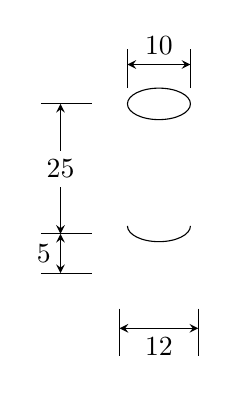
\begin{tikzpicture}[>=stealth]
\tkzDefPoints{0/0/A, 1/0/B, 1.35/.35/C, 1/.7/D, 0/.7/E, -.35/.35/F, 0/.5/A'}
\foreach \x in {B,C,D,E,F}
{
    \tkzDefPointBy[translation = from A to A'](\x)  \tkzGetPoint{\x'}
}
\tkzDrawSegments[](A,A' B,B' C,C' F',F A,B B,C F,A A',B' B',C' C',D' E',F' F',A')

\tkzDefPoints{.1/.95/M, .9/.95/N, .1/2.5/M', .9/2.5/N'}
\tkzDrawSegments[](M,M' N,N')
\draw(.5,2.5)ellipse(.4 and .2);
\draw(.9,.95) arc [start angle =0, end angle =-180, x radius=.4, y radius=.2];
\tkzInterLL(M,M')(D',E') \tkzGetPoint{tmp1}
\tkzInterLL(N,N')(D',E') \tkzGetPoint{tmp2}
\tkzDrawSegments[](D',tmp2 E',tmp1)

\draw[<->](.1,3)--node[above]{$10$}(.9,3);
\draw[<->](0,-.35)--node[below]{$12$}(1,-.35);
\draw[<->](-.75,.85)--node[fill=white]{$25$}(-.75,2.5);
\draw[<->](-.75,.85)--node[left]{$5$}(-.75,.35);
\foreach \x in {.85, 2.5, .35}
{
    \draw(-1,\x)--(-.35,\x);
}
\foreach \x in {0,1}
{
    \draw(\x,-.1)--(\x,-.7);
}
\foreach \x in {0.1,.9}
{
    \draw(\x,2.7)--(\x,3.2);
}
\end{tikzpicture}
\captionof*{figure}{第7题}
\end{minipage}

\item 用油漆涂100个圆台形水桶，桶口直径为30cm，桶底直径为25cm，母线长是27.5cm；已知每平方米需要油漆150g．共需油漆多少kg?
\item 已知：圆台上、下底面面积是$S'$、$S$，中截面面积为$S_0$. 

求证：$2\sqrt{S_0}=\sqrt{S}+\sqrt{S'}$
\end{enumerate}

\begin{center}
    \bfseries B
\end{center}

\begin{enumerate}\setcounter{enumi}{10}
    \item 已知圆锥$S-ABC$的母线和底面所成的角为$\alpha$，$AB$为底面圆的直径，$C$为$\wideparen{AB}$的中点，设二面角为$A-SC-B$等于
$\beta$

求证：$\cos\beta=\frac{\cos^2\alpha}{\cos^2\alpha-2}$

\noindent
\begin{minipage}{.6\textwidth}
\item 从一个底面半径和高都是$R$的圆柱中，挖去一个以圆柱上底面为底，下底面中心为顶点的圆锥得到一个如右图的几何体。如果用一个与圆柱下底面距离等于$d$并且平行于底面的平面去截它，求截面面积.
\end{minipage}
\hfill
\begin{minipage}{.38\textwidth}
\centering
\begin{tikzpicture}[]
\tkzDefPoints{0/0/O, 1.5/0/A, -1.5/0/A', 1.5/1.5/B, -1.5/1.5/B', 0/1.5/O'}
\draw[very thick](O') ellipse (1.5 and .4);
\draw[dashed](A) arc [start angle =0, end angle =180, x radius=1.5, y radius=.4];  
\draw[very thick](A) arc [start angle =0, end angle =-180, x radius=1.5, y radius=.4];  

\tkzDrawSegments[dashed](B,O B',O)
\tkzDrawPoints(O')
\tkzDrawSegments[very thick](A',B' A,B)
\end{tikzpicture}
\captionof*{figure}{第12题}
\end{minipage}
\end{enumerate}


\begin{center}
    \bfseries C
\end{center}

\begin{enumerate}\setcounter{enumi}{12  }
    \item 将一个半径为4的半圆面卷成圆锥的侧面。
\begin{enumerate}[(1)]
\item 求这个圆锥的母线和高的夹角；
\item 将所得到的圆锥在平面上绕它的顶点滚动一周，求这圆锥的高所形成的旋转面的面积。
\end{enumerate}
\end{enumerate}

\begin{figure}[htp]
    \centering
\begin{tikzpicture}
\begin{scope}[rotate=10]
\draw(60:2) arc (60:60+180:2);
\draw(60:2)--(60+180:2);
\draw(0,0)--(-60:2);
\draw[dashed](-60:2) arc [start angle =0, end angle =180, x radius=1, y radius=.4];
\draw[very thick](-60:2) arc [start angle =0, end angle =-180, x radius=1, y radius=.4];
\tkzDefPoint(60+180:2){B}
\tkzDefPoint(-60:2){A}
\tkzDefMidPoint(A,B) \tkzGetPoint{O_1}
\tkzDefPoints{0/0/O}
\tkzDrawSegments[dashed](O,O_1 A,B)
\tkzLabelPoints[left](O)
\tkzLabelPoints[below](O_1)
\node at (60:1)[right]{$R$};
\tkzDefMidPoint(B,O_1) \tkzGetPoint{C}
\node at (C)[above]{$r$};
\end{scope}
\begin{scope}[xshift=6cm, scale=1.3, yshift=-1cm]
\tkzDefPoints{2/0/A1, -2/0/A2, 0/0/O}
\tkzDefPoint(60:2){B1}
\tkzDefPoint(180-60:2){B2}
\tkzDrawSegments[very thick](O,A1 O,A2 O,B1 O,B2)
\tkzDefMidPoint(A1,B1) \tkzGetPoint{C1}
\tkzDefMidPoint(A2,B2) \tkzGetPoint{O_1}
\tkzDefMidPoint(O_1,C1) \tkzGetPoint{O_2}
\draw[rotate=-60, fill=white] (C1) ellipse (1 and .3);
\draw[rotate=60, fill=white] (O_1) ellipse (1 and .3);
\tkzDrawSegments[dashed](O,C1 O,O_1 O,O_2 O_1,C1)
\draw[dashed] (O_2) ellipse (1.45 and .3);
\tkzLabelPoints[below](O_1, O)
\tkzLabelPoints[above](O_2)

\end{scope}
\end{tikzpicture}
    \captionof*{figure}{第13题}
\end{figure}

\section{球}
\subsection{球的概念和性质}
常见的排球、足球及滚珠等物体，都呈球的形象.

\begin{thm}{定义}
    半圆以它的直径为旋转轴，旋转一周所成的曲面叫做\textbf{球面}. 球面所围成的几何体叫做\textbf{球体}，简称\textbf{球}. 旋转出球面的半圆的圆心叫做\textbf{球心}，连结球心和球面上任意一点的线段叫做\textbf{球的半径}. 连结球面上两点并且经过球心的线段叫做\textbf{球的直径}．
\end{thm}

\noindent
\begin{minipage}{.68\textwidth}\CTEXindent
如图2.60的球中，点$O$是球心，线段$OC$是球的半径，线段$AB$是球的直径.

球面也可以看作到定点的距离等于定长的所有点的集合.这里，定点就是球心，定长就是球的半径的长.

一个球用表示它的球心的字母来表示，例如球$O$.
\end{minipage}
\hfill
\begin{minipage}{.3\textwidth}
\centering
\begin{tikzpicture}[scale=1.4]
\draw[very thick](0,0)node[right]{$O$}circle (1);
\draw[very thick] (1,0) arc [start angle =0, end angle =-180, x radius=1, y radius=.35];
\draw[dashed] (1,0) arc [start angle =0, end angle =180, x radius=1, y radius=.35];
\tkzDefPoint(70:1){C}
\draw[dashed, rotate=70](C) arc [start angle =0, end angle =-180, x radius=1, y radius=.35];  
\draw[thick, rotate=70](C) arc [start angle =0, end angle =180, x radius=1, y radius=.35]; 
\tkzDefPoints{0/0/O, 0/.7/A, 0/-.7/B, -.45/-.35/C}
\tkzLabelPoints[right](A,B)
\tkzDrawPoints(A,B,O)
\tkzDrawSegments[dashed](A,B)
\draw[dashed](O)--node[above]{$R$}(C)node[below left]{$C$};

\end{tikzpicture}
\captionof{figure}{}
\end{minipage}



球有下列一些性质：
\begin{enumerate}[(1)]
\item 同球的所有半径（或直径）相等．
\item 球被平面所截，截面是一个圆面． 
\end{enumerate}

性质（1）可由球的定义直接推出，现在证明性质（2）．

已知：球$O$被平面$\alpha$所截.

求证：截面是一个圆面.

\begin{proof}
设球$O$的半径是$R$，球$O$的球面与平面$\alpha$的交线是$\ell$.
\begin{enumerate}[(1)]
\item 平面$\alpha$过球心$O$．如图2.61．

设$A$在$\ell$上任一点. 因为$A$点在球面上，所以$OA=R$. 又$A$在$\alpha$内所以$A$点在$\alpha$内以$O$点为圆心，$R$为半径的圆上.

设$B$是平面$\alpha$内以$O$点为圆心，$R$为半径的圆上的任意一点.

$\because\quad OB=R$, 

$\therefore\quad $点$B$在球面上，从而点$B$是平面$\alpha$与球面的公共点，故点$B$在球面与平面$\alpha$的交线$\ell$上.

所以$\ell$就是平面$\alpha$内以$O$为圆心，以$R$为半径的圆.

\noindent
\begin{minipage}{.47\textwidth}
\centering
\begin{tikzpicture}[scale=1.4]
\tkzDefPoints{0/0/A, 3/0/B, 4/1.5/C, 1/1.5/D, 2/.8/O, 3/.8/A1, 1/.8/A2}
\tkzDrawSegments[](A,B B,C D,A)
\draw[very thick](A1)arc(0:180:1); 
\draw[very thick] (A1) arc [start angle =0, end angle =-180, x radius=1, y radius=.45];
\draw[dashed] (A1) arc [start angle =0, end angle =180, x radius=1, y radius=.45];
\tkzInterLC(A,B)(O,A1)  \tkzGetPoints{tmp1}{tmp2}
\tkzInterLC(C,D)(O,A1)  \tkzGetPoints{tmp3}{tmp4}
\tkzDrawArc[black](O,tmp2)(tmp1)
\tkzDrawArc[dashed, black](O,tmp2)(A1)
\tkzDrawArc[dashed, black](O,A2)(tmp1)
\tkzDrawSegments[](tmp3,D tmp4,C)
\tkzDrawSegments[dashed](tmp3,tmp4)
\tkzDrawPoints(O)
\tkzLabelPoints[right](O)
\tkzLabelAngle[pos=.4](B,A,D){$\alpha$}

\end{tikzpicture}
\captionof{figure}{}
\end{minipage}
\hfill
\begin{minipage}{.47\textwidth}
\centering
\begin{tikzpicture}[scale=1.4]
\tkzDefPoints{0/0/A, 3/0/B, 4/1.5/C, 1/1.5/D, 2/.8/O, 2+.92/.8-.4/A1, 2-.92/.8-.4/A2}
\tkzDrawSegments[](A,B B,C D,A)
  
\draw[very thick] (A1) arc [start angle =0, end angle =-180, x radius=.92, y radius=.2];
\draw[dashed] (A1) arc [start angle =0, end angle =180, x radius=.92, y radius=.2];
\tkzDrawArc[black, thick](O,A1)(A2)
\tkzDefMidPoint(A1,A2) \tkzGetPoint{O_1} 
\tkzInterLC(C,D)(O,A1)  \tkzGetPoints{tmp3}{tmp4}
\tkzDrawSegments[](tmp3,D tmp4,C)
\tkzDrawSegments[dashed](tmp3,tmp4)
\tkzDrawPoints(O)
\tkzLabelPoints[above](O)
\tkzLabelPoints[below](O_1)
\tkzLabelAngle[pos=.4](B,A,D){$\alpha$}

\tkzInterLC(A,B)(O,A1)  \tkzGetPoints{tmp1}{tmp2}
\tkzDrawArc[black](O,tmp2)(tmp1)
\tkzDrawArc[dashed, black](O,tmp2)(A1)
\tkzDrawArc[dashed, black](O,A2)(tmp1)


\tkzDefPoints{1.5/.2/A, 2.5/.2/B}

\tkzDrawSegments[dashed](O,O_1 O,A O,B O_1,A O_1,B)
\tkzLabelPoints[above](A,B)
\end{tikzpicture}
\captionof{figure}{}
\end{minipage}

\item 平面$\alpha$不过球心．

自球心$O$作$OO_1$垂直于平面$\alpha$，垂足是$O_1$. 设$OO_1=d$, 设$A$是$\ell$上任意一点. 

$\because\quad O_1A\subset \alpha$

$\therefore\quad OO_1\bot O_1A$

$\because\quad O_1A=\sqrt{OA^2-OO_1^2}=\sqrt{R^2-d^2}$

$\therefore\quad $点$A$在平面$\alpha$内以$O_1$为圆心，以$\sqrt{R^2-d^2}$为半径的圆上.

设点$B$是平面$\alpha$内以$O_1$为圆心，以$\sqrt{R^2-d^2}$为半径的圆上的任意一点，连结$O_1B$、$OB$.

$\because\quad OO_1\bot \alpha, \quad O_1\subset\alpha$

$\therefore\quad OO_1\bot O_1B$

在${\rm Rt}\triangle OO_1B$中，$$OB=\sqrt{OO_1^2+O_1B^2}=\sqrt{d^2+R^2-d^2}=R$$

$\therefore\quad B$点在球$O$的球面上，故点$B$在球面与平面$\alpha$的交线$\ell$上.

$\therefore\quad \ell$就是平面$\alpha$内以$O_1$为圆心，以$\sqrt{R^2-d^2}$为半径的圆.
\end{enumerate}
综合（1）、（2）无论$\alpha$是否过球心，截面都是圆面．
\end{proof}
 
球的截面有以下性质：
\begin{thm}
    {定理1} 球心和截面圆心的连线垂直于截面．
\end{thm}

已知：$O$和$O'$分别是球$O$和截面圆的球心和圆心

求证：$OO'$垂直于截面.

\begin{proof}
作圆$O'$的两条直径$AB$、$CD$，则$O'A=O'B$,

\noindent
\begin{minipage}{.6\textwidth}\CTEXindent
$\because\quad A$、$B$在球面上，

$\therefore\quad OA=OB$.

在等腰三角形$OAB$中，$O'$
是底边$AB$上的中线，

$\therefore\quad OO'$也是$AB$边上的高，

$\therefore\quad OO'\bot AB$.

同理$OO'\bot CD$，而$AB$、$CD$是截面圆中两条相交直线.
\end{minipage}
\hfill
\begin{minipage}{.38\textwidth}
\centering
\begin{tikzpicture}[]
\tkzDefPoints{0/0/O, -.5/-1.4/A, 0/-1/O', .5/-.6/B, 1.73/-1/A1}
\draw[very thick](O) circle(2)  ;
\draw[very thick] (A1) arc [start angle =0, end angle =-180, x radius=1.73, y radius=.4];
\draw[dashed] (A1) arc [start angle =0, end angle =180, x radius=1.73, y radius=.4];
\tkzDrawSegments[dashed](O,A O,B A,B O,O')

\tkzDefPoints{-.75/-.65/C, .75/-1.35/D}
\tkzDrawSegments[dashed](C,D)
\tkzLabelPoints[above](O,C)
\tkzLabelPoints[above left](A)
\tkzLabelPoints[above right](B)
\tkzLabelPoints[right](O')
\tkzLabelPoints[below](D)

\end{tikzpicture}
\captionof{figure}{}
\end{minipage}


$\therefore\quad OO'$垂直于截面．
\end{proof}

\begin{thm}
{定理2} 球心到球的截面的距离$d$与球的半径$R$，及截面
圆的半径$r$有下面关系：
\[r=\sqrt{R^2-d^2}\]    
\end{thm}

本定理可直接由定理1推出，请读者自己证明．

\begin{thm}
    {推论1} 与球心距离相等的截面，所截得的圆大小相等．
\end{thm}


\begin{thm}
    {推论2} 与球心距离不等的截面，所截得的圆大小不等．距离球心较近的截面所截得的圆较大.
\end{thm}


\begin{thm}
    {推论3} 当$d=0$时，截面过球心，$r=R$. 截面圆最大.
\end{thm}


\begin{thm}
    {推论4} 当$d=R$时，$r=0$，截面缩成一个点.
\end{thm}

下面介绍几个与球面有关的概念：

当截面过球心时，球面被截得的圆叫做\textbf{球的大圆}（图2.64).

球面被不经过球心的截面截得的圆叫做\textbf{球的小圆}（图2.65).


\noindent
\begin{minipage}{.47\textwidth}
\centering
\begin{tikzpicture}[scale=1.4]
\tkzDefPoints{0/0/A, 3/0/B, 4/1.5/C, 1/1.5/D, 2/.8/O, 3/.8/A1, 1/.8/A2}
\tkzDrawSegments[](A,B B,C D,A)
\draw[very thick](A1)arc(0:180:1); 
\draw[very thick] (A1) arc [start angle =0, end angle =-180, x radius=1, y radius=.45];
\draw[dashed] (A1) arc [start angle =0, end angle =180, x radius=1, y radius=.45];
\tkzInterLC(A,B)(O,A1)  \tkzGetPoints{tmp1}{tmp2}
\tkzInterLC(C,D)(O,A1)  \tkzGetPoints{tmp3}{tmp4}
\tkzDrawArc[black](O,tmp2)(tmp1)
\tkzDrawArc[dashed, black](O,tmp2)(A1)
\tkzDrawArc[dashed, black](O,A2)(tmp1)
\tkzDrawSegments[](tmp3,D tmp4,C)
\tkzDrawSegments[dashed](tmp3,tmp4)
\tkzDrawPoints(O)
\tkzLabelPoints[right](O)
\tkzLabelAngle[pos=.4](B,A,D){$\alpha$}
\draw[dashed](O)--node[above]{$R$}+(-1,0);
\end{tikzpicture}
\captionof{figure}{}
\end{minipage}
\hfill
\begin{minipage}{.47\textwidth}
\centering
\begin{tikzpicture}[scale=1.4]
\tkzDefPoints{0.3/0/A, 3/0/B, 3.5/1/C, .8/1/D, 2/.8/O, 2+.92/.8-.4/A1, 2-.92/.8-.4/A2}
\tkzDrawSegments[](A,B B,C D,A)
  
\draw[very thick] (A1) arc [start angle =0, end angle =-180, x radius=.92, y radius=.2];
\draw[dashed] (A1) arc [start angle =0, end angle =180, x radius=.92, y radius=.2];
\tkzDrawArc[black, thick](O,A1)(A2)
\tkzDefMidPoint(A1,A2) \tkzGetPoint{O'} 
\tkzInterLC(C,D)(O,A1)  \tkzGetPoints{tmp3}{tmp4}
\tkzDrawSegments[](tmp3,D tmp4,C)
\tkzDrawSegments[dashed](tmp3,tmp4)
\tkzDrawPoints(O)
\tkzLabelPoints[above](O)
\tkzLabelPoints[right](O')
\tkzLabelAngle[pos=.4](B,A,D){$\alpha$}

\tkzInterLC(A,B)(O,A1)  \tkzGetPoints{tmp1}{tmp2}
\tkzDrawArc[black](O,tmp2)(tmp1)
\tkzDrawArc[dashed, black](O,tmp2)(A1)
\tkzDrawArc[dashed, black](O,A2)(tmp1)
\tkzDefPoints{1.5/.24/A}
\tkzDrawSegments[dashed](O,O' O',A)
\draw[dashed](O)--node[left]{$R$}(A);
\draw[dashed](O)--node[right]{$d$}(O');

\end{tikzpicture}
\captionof{figure}{}
\end{minipage}

当平面和球面有且只有一个公共点时，叫做平面和球相切，这个平面叫做球的切面，球与它的切面的公共点叫做\textbf{切点}.

连结球面上$A$、$B$两点间的大圆的劣弧长叫做球面上$A$、$B$两点间的\textbf{球面距离}（它是球面上$A$、$B$两点间的最短距离）.

\begin{thm}
    {定理} 如果球的半径通过球的切面的切点，则这半径垂直于球的切面。
\end{thm}

已知：平面$\alpha$与球$O$切于$A$点.

求证：$OA\bot \alpha$.

\noindent
\begin{minipage}{.6\textwidth}
\begin{proof}
    如图2.66，设球的半径是$R$，假设$OA$与平面$\alpha$不垂直. 则可过$O$点作$\alpha$的垂线$OA'$，垂足是$A'$，因为从平面外一点作平面的垂线段和斜线段中，垂线段最短，故$OA'<OA$，即$OA'<R$。这样$A'$点就在球的内部，
平面$\alpha$与球$O$必然不只有一个公共点，这与$\alpha$与球$O$相切矛盾，所以$OA\bot\alpha$.
\end{proof}
\end{minipage}
\hfill
\begin{minipage}{.38\textwidth}
\centering
\begin{tikzpicture}[scale=1.2]
    \tkzDefPoints{0/0/A1, 3.5/0/B1, 4/1/C1, .5/1/D1, 2/1.5/O, 2/.3/A}
\tkzDrawSegments[very thick](A1,B1 B1,C1 D1,A1)
\tkzInterLC(C1,D1)(O,A) \tkzGetPoints{tmp1}{tmp2}
\tkzDrawSegments[very thick](C1,tmp1 D1,tmp2)
\draw[very thick](O) circle(1.2);
\tkzLabelAngle[pos=.5](B1,A1,D1){$\alpha$}
\tkzDefPoints{3.2/1.5/A'}
\draw[very thick] (A') arc [start angle =0, end angle =-180, x radius=1.2, y radius=.4];
\draw[dashed] (A') arc [start angle =0, end angle =180, x radius=1.2, y radius=.4];
\draw[dashed](A)node[above left]{$A$}--(O)node[right]{$O$};
\draw[dashed](O)--+(-70:1.2)node[right]{$A'$};
\tkzDrawPoints(O)
\end{tikzpicture}
\captionof{figure}{}
\end{minipage}

\subsection*{2.6 练习1}
\begin{enumerate}
\item 球的与球心距离相等的截面圆的大小有什么关系？这些圆的圆心的轨迹是什么？
\item 求证：球面上任意三点$A$、$B$、$C$都不可能在一条直线上.
\item 求证：球的任意两个大圆互相平分．
\item 求证：若两球相交，则两球面的公共点的集合是一个圆.
\item 在半径是13cm的球面上有$A$、$B$、$C$三点，$AB=6$cm，$BC=8$cm，$CA=10$cm，求经过这三点的截面和球心的距离.
\item 在半径为$R$的球面上有$A$、$B$、$C$三点，$AB=BC=CA=a$，求$a$的范围，并求出过$A$、$B$、$C$三点的平面到球心的距离.
\item 球面上有$A$、$B$、$C$、$D$四点，已知$AB\bot AC$，$AC\bot AD$，$AD\bot AB$，且$AB=AC=AD=a$，求这球的半径.
\end{enumerate}

\subsection{球的直观图的画法}
画球的直观图，一般采用正等测画法.

\begin{example}
画半径为$R$的球的直观图.
\end{example}

\begin{solution}
\textbf{画法：}
\begin{enumerate}[(1)]
\item 画轴．过点$O$画$x$轴、$y$轴、$z$轴，使每两个轴的正向成$120^{\circ}$角；
\item 画大圆．以$O$为中心，在每两个轴确定的平面内，画半径为$R$的圆的直观图（三个椭圆）
\item 成图．以$O$点为圆心，画一个与上述三个椭圆都相切的圆．整理后就得到半径为$R$的球的直观图（图2.67）．
\end{enumerate}
\end{solution}

\begin{note}
画球的直观图时，为了简便，通常用下述方法来画半径为$R$的圆的直观图.
\begin{enumerate}[(1)]
    \item 画半径为$R$的圆；
    \item 在这个圆内画一个（或两个）椭圆（使椭圆的长轴等于$2R$）与这圆相切（图2.68甲、乙）．
\end{enumerate}
\end{note}

\noindent
\begin{minipage}{.3\textwidth}
\centering
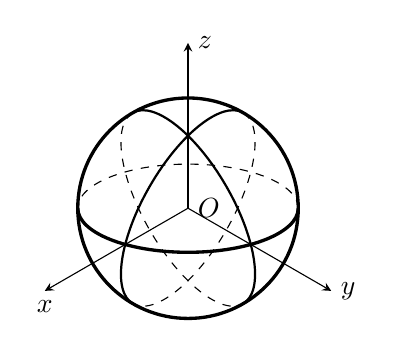
\begin{tikzpicture}[scale=.7, >=stealth]
\draw[->](0,0)node[right]{$O$}--(0,3)node[right]{$z$};
\draw[->](0,0)--(-30:3)node[right]{$y$};
\draw[->](0,0)--(-150:3)node[below]{$x$};
\draw[very thick](0,0) circle(2);
\draw[very thick] (2,0) arc [start angle =0, end angle =-180, x radius=2, y radius=.8];
\draw[dashed] (2,0) arc [start angle =0, end angle =180, x radius=2, y radius=.8];

\draw[dashed, rotate=60] (2,0) arc [start angle =0, end angle =-180, x radius=2, y radius=.8];
\draw[thick, rotate=60] (2,0) arc [start angle =0, end angle =180, x radius=2, y radius=.8];

\draw[thick, rotate=120] (2,0) arc [start angle =0, end angle =-180, x radius=2, y radius=.8];
\draw[dashed, rotate=120] (2,0) arc [start angle =0, end angle =180, x radius=2, y radius=.8];

\foreach \x/\y in {90/C, -150/A, -30/B}
{
    \tkzDefPoint(\x:1.3){\y}
    \tkzDrawPoints(\y)
}
\tkzLabelPoints[right](C)
\tkzLabelPoints[left](A)
\tkzLabelPoints[right](B)


\end{tikzpicture}
\captionof{figure}{}
\end{minipage}
\hfill
\begin{minipage}{.65\textwidth}
\centering
\begin{tikzpicture}[]
\begin{scope}
\tkzDefPoints{0/0/O}
\draw[very thick](O) circle (1.5);
\draw[very thick] (1.5,0) arc [start angle =0, end angle =-180, x radius=1.5, y radius=.6];
\draw[dashed] (1.5,0) arc [start angle =0, end angle =180, x radius=1.5, y radius=.6];

\draw[dashed, rotate=90] (1.5,0) arc [start angle =0, end angle =-180, x radius=1.5, y radius=.6];
\draw[thick, rotate=90] (1.5,0) arc [start angle =0, end angle =180, x radius=1.5, y radius=.6];
\tkzDrawPoints(O)
\node at (0,-2){甲};
\end{scope}
\begin{scope}[xshift=4cm]
\tkzDefPoints{0/0/O}
\draw[very thick](O) circle (1.5);
\draw[very thick] (1.5,0) arc [start angle =0, end angle =-180, x radius=1.5, y radius=.6];
\draw[dashed] (1.5,0) arc [start angle =0, end angle =180, x radius=1.5, y radius=.6];

\tkzDrawPoints(O)
\node at (0,-2){乙};
\end{scope}
\end{tikzpicture}
\captionof{figure}{}
\end{minipage}

在地球仪上我们可以看到许多纵横交错的曲线，这是人
们为了表示地球表面上某点的位置，引入了经线和纬线的概念. 这同为了表示平面上点的位置建立平面坐标系类似（图2.69)。

\begin{figure}[htp]
    \centering
\begin{tikzpicture}[scale=1.2]

\tkzDefPoints{-2/0/A, 2/0/A', 0/2/B, 0/-2/B'}

\foreach \x in {20,40,60}
{
    \draw[very thick](\x:2)--(180-\x:2)node[left]{$\x^{\circ}$};
    \draw[very thick](-\x:2)--(-180+\x:2)node[left]{$\x^{\circ}$};
}

\draw[dashed](66.5:2)node[right=.1]{$\left(66\tfrac{1}{2}\right)^{\circ}$北极圈}--(180-66.5:2);
\draw[dashed](-66.5:2)node[right=.1]{$\left(66\tfrac{1}{2}\right)^{\circ}$南极圈}--(-180+66.5:2);

\draw[dashed](23.5:2)node[right=.1]{$\left(23\tfrac{1}{2}\right)^{\circ}$北回归线}--(180-23.5:2);
\draw[dashed](-23.5:2)node[right=.1]{$\left(23\tfrac{1}{2}\right)^{\circ}$南回归线}--(-180+23.5:2);

\draw[very thick](B') arc (-75:75:2.06);
\draw[very thick](B) arc (180-75:180+75:2.06);

\draw[very thick](B') arc (-40:40:3.1);
\draw[very thick](B) arc (180-40:180+40:3.1);
\draw[very thick](B)node[above]{$90^{\circ}$}--(B')node[below]{$90^{\circ}$};
\node [fill=white]at (0,0)[above]{$90^{\circ}$};
\node [fill=white]at (.7,0)[above]{$120^{\circ}$};
\node [fill=white]at (-.7,0)[above]{$60^{\circ}$};
\node [fill=white]at (1.6,0)[above]{$150^{\circ}$};
\node [fill=white]at (-1.6,0)[above]{$30^{\circ}$};
\draw[very thick](A)node[left]{$0^{\circ}$}--(A')node[right]{赤道};

\draw[very thick](0,0)circle(2);

\end{tikzpicture}
    \caption{}
\end{figure}

把地球看作一个球时，经线就是从北极到南极的半个大圆. 这样除了南、北极外，在地球球面上每一点就有且只有一条经线，为了区别不同经线的位置，又引入了度的概念；把经过英国格林威治天文台的经线作为$0^{\circ}$经线．如果某地$P$在$0^{\circ}$经线以东，它所在的经线平面与$0^{\circ}$经线所在的平面之间的二面角的度数$\alpha$就是过$P$点的经线的度数（图2.70甲），说这条经线是东经$\alpha^{\circ}$的经线．东经最大$180^{\circ}$，它是与$0^{\circ}$经线在同一平面中的经线，和$0^{\circ}$经线构成一个大圆．同样规定西经经线的度数．西经经线的度数最大是西经$180^{\circ}$，它与东经$180^{\circ}$是同一条经线．

赤道是过地球球心且与地轴垂直的平面与地球表面的交线（是个大圆），称为$0^{\circ}$纬线，凡是与赤道平面平行的平面截地球表面所得的圆（都是小圆）都是纬线. 这样过地球表面
上任一点都有一条纬线.纬线的度数，就是这纬线上任一点的球半径与赤道平面夹角的度数$\theta$（图2.70乙），如果 这条纬线在赤道以北，就说这条纬线是北纬$0^{\circ}$纬线．显然$0^{\circ}\le \theta\le 90^{\circ}$.

\begin{figure}[htp]
    \centering
\begin{tikzpicture}
\begin{scope}
\tkzDefPoints{0/0/O, 2/0/a, 0/1.75/N}
\draw[very thick](a) arc (0:180:2);
\draw[dashed](a) arc [start angle =0, end angle =180, x radius=2, y radius=1];
\draw[very thick](a) arc [start angle =0, end angle =-180, x radius=2, y radius=1];
\node at (0,-1.5){甲};
\tkzDefPoints{-1.6/-.6/A, -.5/-.95/B, -.5/.5/P}
\tkzDrawSegments[dashed](O,A O,B N,O)
\tkzLabelPoints[below](A,B)
\draw[very thick](N)[bend left=-30] to (A);
\draw[very thick](N)[bend left=-20] to (B);
\node at (0,0.7)[right]{地轴};
\node at (1.3,-.75)[below]{赤道};
\tkzMarkAngles[size=.3, mark=none](A,O,B)
\tkzLabelAngle[pos=.45](A,O,B){$\alpha$}
\tkzDrawPoints(P)
\tkzLabelPoints[right](O,N,P)
\node at (0,-2.5)[text width=5cm]{$\wideparen{NA}$是$0^{\circ}$经线，$P$点的经度是二面角$A-NO-B$的度数};


\end{scope}
\begin{scope}[xshift=6cm]
    \tkzDefPoints{0/0/O, 2/0/a, 0/1.75/N}
\draw[very thick](a) arc (0:180:2);
\draw[dashed](a) arc [start angle =0, end angle =180, x radius=2, y radius=1];
\draw[very thick](a) arc [start angle =0, end angle =-180, x radius=2, y radius=1];
\node at (0,0.7)[right]{地轴};
\node at (0,-1.5){乙};
\tkzDefPoints{-1.3/-.75/A, -.7/1.15/P}
\tkzDrawSegments[dashed](O,A   N,O)
\tkzLabelPoints[right](O,N)
\tkzLabelPoints[below](A)
\draw[very thick](N)[bend left=-30] to (A);
\node at (1.3,-.75)[below]{赤道};
\tkzDrawPoints(P)
\tkzLabelPoints[above left](P)
\tkzDrawSegments[](P,O)
\tkzMarkAngles[size=.3, mark=none](P,O,A)
\tkzLabelAngle[pos=.45](P,O,A){$\theta$}

\node at (0,-2.5)[text width=5cm]{$\wideparen{NA}$是某一经线，$P$点的纬度是$\angle POA$的度数};
\end{scope}
\end{tikzpicture}
    \caption{}
\end{figure}

\begin{example}
    设地球的半径为$R$，在北纬$30^{\circ}$圈上有$A$、$B$两地．
\begin{enumerate}[(1)]
\item 它们的经度相差$120^{\circ}$．求经过这两地的纬线的长．
\item 若它们经度相差$180^{\circ}$，求$A$、$B$两地的球面距离．
\end{enumerate}
\end{example}

\begin{solution}
\begin{enumerate}[(1)]
    \item 如图2.71，设过$B$点的经线与赤道交于$D$点，则$\angle BOD=30^{\circ}$.
    
设$O'$是$30^{\circ}$纬度圈的圆心，则$BO'\bot OO'$. 
在${\rm Rt}\triangle OO'B$中，
$$O'B=OB\cdot \cos\angle OBO'=R\cdot \cos\angle BOD=R\cdot \cos30^{\circ}=\frac{\sqrt{3}}{2}R$$
即$30^{\circ}$纬度圈这个圆的半径是$\frac{\sqrt{3}}{2}R$.

$\because\quad A$、$B$两地经度相差$120^{\circ}$，

$\therefore\quad \angle AO'B=120^{\circ}$

$\therefore\quad $经过$A$、$B$两地的纬线长是
\[2\pi \cdot O'B\cdot \frac{120}{360}=2\pi \cdot \frac{\sqrt{3}}{2}R\cdot \frac{1}{3}=\frac{\sqrt{3}}{3}\pi R\]

\noindent
\begin{minipage}{.45\textwidth}
\centering
\begin{tikzpicture}[]
    \tkzDefPoints{0/0/O, -2/0/C, 0/1/O', 0/2/O''}
    \tkzDefPoint(150:2){A}
    \tkzLabelPoints[left](A,C)
    \tkzDrawSegments[dashed](C,O A,O' O,O'')
    \draw[very thick](O) circle (2);
    \draw[very thick] (C) arc [start angle =180, end angle =360, x radius=2, y radius=.6];
    \draw[dashed] (C) arc [start angle =180, end angle =0, x radius=2, y radius=.6];
    \draw[very thick] (A) arc [start angle =180, end angle =360, x radius=1.732, y radius=.4];
    \draw[dashed] (A) arc [start angle =180, end angle =0, x radius=1.732, y radius=.4];
    \draw[very thick] (O'') arc [start angle =90, end angle =-90, x radius=.6, y radius=2];
\tkzDefPoints{.6/-.6/D, .6/.6/B}
\tkzDrawSegments[dashed](B,O' D,O)
\tkzLabelPoints[below right](B,D)
\tkzLabelPoints[below](O)
\tkzLabelPoints[right](O')

\end{tikzpicture}
\captionof{figure}{}
\end{minipage}
\hfill
\begin{minipage}{.45\textwidth}
\centering
\begin{tikzpicture}[]
    \tkzDefPoints{0/0/O, -2/0/C, 0/1/O', 0/2/O''}
    \draw[very thick](O) circle (2);
    \tkzDefPoint(150:2){A}
    \tkzDefPoint(30:2){B}
    \draw[very thick] (A) arc [start angle =180, end angle =360, x radius=1.732, y radius=.4];
    \draw[dashed] (A) arc [start angle =180, end angle =0, x radius=1.732, y radius=.4];
    \tkzDrawSegments[dashed](A,B O,O'' O,A O,B)
    \tkzLabelPoints[left](A)
    \tkzLabelPoints[right](B)
\tkzLabelPoints[below](O)
\draw[very thick] (C) arc [start angle =180, end angle =360, x radius=2, y radius=.6];
\draw[dashed] (C) arc [start angle =180, end angle =0, x radius=2, y radius=.6];
\tkzLabelPoints[right](O')
\tkzMarkAngles[size=.2, mark=none](B,O,A)
\tkzLabelAngle[pos=.4](B,O,A){$\theta$}


\end{tikzpicture}
\captionof{figure}{}
\end{minipage}
    
\item $\because\quad A$、$B$经度相差$180^{\circ}$，

$\therefore\quad$线段$AB$的长是$AB=2O'B=\sqrt{3}R$.

在过$A$、$B$两点的大圆中，$OA=OB=R$, $AB=\sqrt{3}R$. 设$AB$弦所对的圆心角为$\theta$，则
\[\cos\theta=\frac{OA^2+OB^2-AB^2}{2OA\cdot OB}=\frac{-R^2}{2R^2}=-\frac{1}{2}\]

$\therefore\quad \theta=\frac{2}{3}\pi$

$\therefore\quad AB$两地的球面距离是$R\theta=\frac{2}{3}\pi R$.


\end{enumerate}
\end{solution}

\begin{remark}
    求球面上两点间的距离，一般要求以这两点为端点的半径的夹角，而这角又经常通过弦$AB$的长度来求.
\end{remark}

\subsection*{2.6 练习2}
一、解答题：
\begin{enumerate}
\noindent
\begin{minipage}{.7\textwidth}
\item 在下图中，设$\wideparen{NAS}$是$0^{\circ}$经线。
\begin{enumerate}[(1)]
\item 标出位于东经$116^{\circ}$，北纬$20^{\circ}$的地点$P$的位置．
\item 标出位于东经$180^{\circ}$上的赤道上一点$Q$的位置.
\item 标出位于西经$180^{\circ}$，南纬$45^{\circ}$的一点$M$的位置．
\end{enumerate} 
\end{minipage}
\hfill
\begin{minipage}{.25\textwidth}
\centering
\begin{tikzpicture}[]
\tkzDefPoints{0/0/O, 0/1/N, 0/-1/S, 1/0/a}
\draw[very thick](O) circle(1);
\tkzDrawSegments[dashed](N,S)
\draw[dashed](a) arc [start angle =0, end angle =180, x radius=1, y radius=.4];
\draw[very thick](a) arc [start angle =0, end angle =-180, x radius=1, y radius=.4];
\tkzLabelPoints[above](N)
\tkzLabelPoints[below](S)
\tkzLabelPoints[right](O)
\draw[very thick](N) to[bend left=-80] (S);
\tkzDefPoints{-.5/-.35/A}
\tkzDrawSegments[dashed](A,O)
\tkzLabelPoints[below left](A)
\tkzDrawPoints(O)
\end{tikzpicture}
\captionof*{figure}{第1题}
\end{minipage}

\item 我国首都北京靠近北纬$40^{\circ}$，求北纬$40^{\circ}$的纬线长度约为多少km（地球半径约6370km）.
\item 海面上，地球球心角$1'$所对的大圆弧长约为1海里，海里约是多少km（地球半径约为6370km）？
\item 为什么飞机和轮船都是尽可能以大圆弧为航线航行？
\end{enumerate}

二、填空题：
\begin{enumerate}
\item 棱长为1的正方体的内切球的半径是外接球的半径是\blank，外接球的面积是\blank.
\item 半径为5cm的球面上有$A$、$B$、$C$三点$AB=6.4$cm, $BC=4.8$cm，$CA=8$cm，则平面$ABC$与球心的距离是\blank.
\item 一个球的两个切面成$120^{\circ}$的二面角，两个切点的球面距离是$12\pi$cm，则这个球的半径是\blank.
\item 一个球的半径为$a$，放在墙角（直三面角），与墙角的三个面都相切，则球心与墙角顶点的距离是\blank.
\item 设地球的半径是$R$，地球的两地$A$、$B$的纬度都是北纬$45^{\circ}$，$A$、$B$两点的球面距离是$\frac{\pi}{3}R$，若$A$在东经$20^{\circ}$处，则$B$点的位置是\blank.
\item $A$位于北纬$30^{\circ}$，地球自转一小时，$A$地转过的路程（地球的半径为$R$）等于\blank.
\item 在半径是5的球面上有两点$A$、$B$，半径$OA$、$OB$夹角是$120^{\circ}$，$A$、$B$两点的球面距离是\blank.
\end{enumerate}


\subsection{球的表面积}
球的表面不能展成平面图形. 所以球的表面积的求法，就不能用圆柱、圆锥那种计算侧面展开图的办法，怎么办
呢？

解决空间问题的方法，一是转化为平面问题，一是用解决平面问题的方法来类比，既然不能用转化成平面图形的办法来求球的表面积，我们就在平面问题中找类似的情况来类比.

在平面几何中，求圆的周长不能用求线段长的方法，而是用它的内接正$n$边形的周长. 当$n$无限增大时，圆的内接正$n$边形的周长和圆的周长的差无限趋于零，从而推出圆周长公式.

我们知道，球是由半圆绕它的直径旋转$360^{\circ}$而得到的，也可看做是由圆绕它的直径旋转$180^{\circ}$而得到的，这时圆的内接正$n$边形可以相应地旋转出圆锥和圆台. 它们的侧面的和，当$n$不断成倍增长时就越来越接近于球面，由此我们想到，能否用球的内接圆台和圆锥的侧面积的和来逼近球的表面积.

怎样用与球有关的量来表示球的内接圆台和内接圆锥的侧面积呢？

圆台的侧面积公式是$S_{\text{圆台侧}}=\pi(r'+r)\ell$，要找这个面积与球的关系，就是要找$(r'+r)$、$\ell$与球的关系.

我们知道球的内接圆台，由圆台的高和母线$\ell$的大小确定. 而$\ell$的大小由它到球心的距离$p$确定，这样由$p$和$h$就确定了球的内接圆台的侧面积，怎么用$p$和$h$来表示圆台的侧面积呢？

\noindent
\begin{minipage}{.6\textwidth}\CTEXindent
    图2.73$ABCD$是球的内接圆台的轴截面，$AD=\ell$, $DO_1=r'$, $AO'_1=r$, $O_1O'_1$是圆台的高$h$. $E$是$AD$的中点，则$OE\bot AD$. 

    过$E$引$EE'\parallel AB$交$O_1O'_1$于$E'$，则$EE'=\frac{1}{2}(r'+r)$.
    
    过$D$作$DD'\bot AB$于$D'$，则$DD'=h$, 且$\triangle DAD'\backsim \triangle EOE'$,
    
    $\therefore\quad AD:DD'=EO:EE'$，
    
    即$\ell: h=p:\frac{1}{2}(r'+r)$.
    
\end{minipage}
\hfill
\begin{minipage}{.36\textwidth}
\centering
\begin{tikzpicture}[scale=.9]
\tkzDefPoints{0/0/O}
\tkzDefPoint(60:2){C}
\tkzDefPoint(180-60:2){D}
\tkzDefPoint(-30:2){B}
\tkzDefPoint(-180+30:2){A}
\tkzDrawPolygon[very thick](A,B,C,D)
\tkzLabelPoints[left](A,D)
\tkzLabelPoints[right](B,C)
\draw[very thick](O)circle (2);
\tkzDefMidPoint(A,B) \tkzGetPoint{O'_1}
\tkzDefMidPoint(C,D) \tkzGetPoint{O_1}
\draw[very thick](O'_1)--(0,2);
\tkzDefMidPoint(A,D) \tkzGetPoint{E}
\tkzDefMidPoint(O_1,O'_1) \tkzGetPoint{E'}

\tkzLabelPoints[right](E',O)
\tkzLabelPoints[left](E)
\tkzDefPointBy[projection= onto A--B](D) \tkzGetPoint{D'}
\tkzDrawSegments[very thick](E,O E,E' D,D')
\tkzLabelPoints[below](O'_1,D')
\tkzLabelPoints[below right](O_1)
\end{tikzpicture}
\captionof{figure}{}
\end{minipage}


$\therefore\quad 2ph=(r'+r)\ell$
    
$\therefore\quad S_{\text{圆台侧}}=\pi(r'+r)\ell=2\pi ph$．

这个公式可以作为定理.

\begin{thm}
    {定理} 球的内接圆台的高为$h$，球心到母线的距离是$p$. 则圆台的侧面积为$2\pi ph$.
\end{thm}

\subsection*{2.6 练习3}
下图甲、乙是球的内接圆柱和圆锥的轴截面图，若圆柱和
圆锥的高为$h$，球心到母线的距离是$p$，用$p\cdot h$表示这圆柱和圆锥的侧面积.
\begin{center}
\begin{tikzpicture}[>=stealth, scale=1.4]
  \begin{scope}
\draw[very thick](0,0) circle (1);
\tkzDefPoint(45:1){A}
\tkzDefPoint(45+90:1){B}
\tkzDefPoint(45+180:1){C}
\tkzDefPoint(45+270:1){D}
\tkzDrawPolygon[very thick](A,B,C,D)
\draw(A)--+(1,0);
\draw(D)--+(1,0);
\draw(O)node[right]{$O$}--node[above]{$p$}+(-.707,0);
\draw[<->](1.5,.707)--node[fill=white]{$h$}(1.5,-.707);
\node at (0,-1.25){甲};
\tkzDrawPoints(O)

\end{scope}
\begin{scope}[xshift=4cm]
\draw[very thick](0,0) circle (1);
\tkzDefPoints{0/0/O}
\node at (0,-1.25){乙};
\tkzDefPoint(90:1){A}
\tkzDefPoint(120+90:1){B}
\tkzDefPoint(240+90:1){C}
\tkzDrawPolygon[very thick](A,B,C)
\draw(A)--+(1.5,0);
\draw(C)--+(.7,0);
\draw[<->](1.25,1)--node[fill=white]{$h$}(1.25,-.5);
\tkzDefPointBy[projection= onto A--B](O) \tkzGetPoint{E}
\draw(O)node[right]{$O$}--node[above]{$p$}(E);
\tkzDrawPoints(O)
\end{scope}  
\end{tikzpicture}
\end{center}

现在，我们来求半径为$R$的球的表面积.

如图2.74，将半球面上的半个大圆$ANB$分成$2n$等分，用
过各分点平行于半球的大圆面的平面将半球分为$n$部分，以截得的圆为底作圆台、圆锥，设它们的高分别是$h_1,h_2,\ldots,h_n$，球心到它们母线的距离是相等的，设为$p$. 由上述定理，这些圆台、圆锥的侧面积的和为
\[\begin{split}
 S&=2\pi ph_1+2\pi ph_2+\cdots +2\pi ph_n\\
&=2\pi p(h_1+h_2+\cdots +h_n)=2\pi pR   
\end{split}\]

\begin{figure}[htp]
    \centering
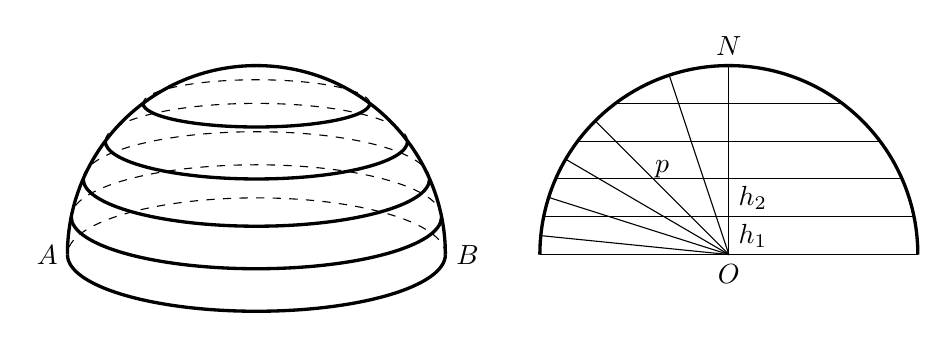
\begin{tikzpicture}[scale=1.2]
\begin{scope}
    \draw[very thick](-2,0) arc (180:0:2);
\tkzDefPoints{0/0/O, 0/2/N, 0/.4/O1, 0/.8/O2, 0/1.2/O3, 0/1.6/O4}
\tkzDrawPoints(O,N,O1,O2,O3,O4)
\tkzLabelPoints[right](O)
\tkzLabelPoints[above](N)
\tkzDrawSegments[dashed](O,N)
\draw[very thick](2,0)node[right]{$B$} arc [start angle =0, end angle =-180, x radius=2, y radius=.6];
\draw[dashed](2,0) arc [start angle =0, end angle =180, x radius=2, y radius=.6];

\draw[very thick](1.96,0.4) arc [start angle =0, end angle =-180, x radius=1.96, y radius=.55];
\draw[dashed](1.96,0.4) arc [start angle =0, end angle =180, x radius=1.96, y radius=.55];

\draw[very thick](1.833,0.8) arc [start angle =0, end angle =-180, x radius=1.833, y radius=.5];
\draw[dashed](1.833,0.8) arc [start angle =0, end angle =180, x radius=1.833, y radius=.5];

\draw[very thick](1.6,1.2) arc [start angle =0, end angle =-180, x radius=1.6, y radius=.4];
\draw[dashed](1.6,1.2) arc [start angle =0, end angle =180, x radius=1.6, y radius=.4];

\node at (-2,0)[left]{$A$};
\draw[very thick](1.2,1.6) arc [start angle =0, end angle =-180, x radius=1.2, y radius=.25];
\draw[dashed](1.2,1.6) arc [start angle =0, end angle =180, x radius=1.2, y radius=.25];

\end{scope}
\begin{scope}[xshift=5cm]
\draw[very thick](-2,0) arc (180:0:2);
\draw(-2,0)--(2,0);
\draw(0,0)node[below]{$O$}--(0,2)node[above]{$N$};
\foreach \x in {11.5, 23.6, 36.9, 53.1}
{
    \draw(\x:2)--(180-\x:2);
}
\foreach \x in {5.75, 17.6, 30.3, 45, 71.6}
{
    \draw(180-\x:2)--(0,0);
}
\node at (0,.2)[right]{$h_1$};
\node at (0,.6)[right]{$h_2$};
\node at (180-45:1)[above]{$p$};

\end{scope}
\end{tikzpicture}
    \caption{}
\end{figure}


当等分点无限增加，侧面就无限地接近于半球面，同时$p$也无限地接近于$R$，当$p$变为$R$时，侧面积的和$S$就变为$2\pi R^2$．我们把这个和作为半球面的面积，由此得到如下定理.

\begin{thm}{定理}
球面面积等于它的大圆面积的4倍，即
\[S_{\text{球面}}=4\pi R^2\]
\end{thm}

\begin{example}
    已知：等边圆柱的底面半径等于球的半径（图2.75）求：
\begin{enumerate}[(1)]
\item 球的表面积与这圆柱侧面积有什么关系？
\item 球的表面积与圆柱的全面积之比是多少？
\end{enumerate}

\end{example}


\begin{solution}

\noindent
\begin{minipage}{.6\textwidth}\CTEXindent
\begin{enumerate}[(1)]
\item 设球的半径为$R$，则圆柱底面半径为$R$，高为$2R$．则$S_{\text{球面}}=4\pi R^2$
\[S_{\text{圆柱侧}}=2\pi R\cdot 2R=4\pi R^2\]

$\therefore\quad S_{\text{球}}=S_{\text{圆柱侧}}$
\item $\because\quad S_{\text{圆柱全}}=4\pi R^2+\pi R^2+\pi R^2=6\pi R^2$,
而$S_{\text{球面}}=4\pi R^2$，

$\therefore\quad \frac{S_{\text{球面}}}{ S_{\text{圆柱全}}}=\frac{4\pi R^2}{6\pi R^2}=\frac{2}{3}$
\end{enumerate}
\end{minipage}
\hfill
\begin{minipage}{.38\textwidth}
\centering
\begin{tikzpicture}[scale=1.4]
\tkzDefPoints{0/0/O, 1/0/A, -1/0/B, 1/1/A1, -1/1/B1, 1/-1/A2, -1/-1/B2}
\draw[dashed](O) circle(1);
\tkzDrawSegments[very thick](B1,B2 A1,A2)
\draw[very thick](0,1) ellipse (1 and .4);
\draw[dashdotted](0,-1.8)--(0,1.8);
\draw[very thick](A2) arc [start angle=0, end angle =-180, x radius=1, y radius=.4];
\draw[dashed](A2) arc [start angle=0, end angle =180, x radius=1, y radius=.4];
\draw[very thick](A) arc [start angle=0, end angle =-180, x radius=1, y radius=.4];
\draw[dashed](A) arc [start angle=0, end angle =180, x radius=1, y radius=.4];
\draw[dashed](B)--node[below]{$R$}(O)node[right]{$O$};

\end{tikzpicture}
\captionof{figure}{}
\end{minipage}
\end{solution}

\begin{example}
    半径为$R$的球内切于圆台，圆台的母线与底面所成角为$\alpha$，求圆台的侧面积与内切球面积之比。
\end{example}

\noindent
\begin{minipage}{.6\textwidth}\CTEXindent
\begin{analyze}
作轴截面如图2.76，设圆台上、下底面半径分别
为$r_1, r_2$，内切球半径为$R$. 则各个量的关系有：
\begin{equation}
   AB=r_1+r_2=\frac{O_1O_2}{\sin\alpha}=\frac{2R}{\sin\alpha}\tag{1} 
\end{equation}
\begin{equation}
    \angle AOB=90^{\circ} \tag{2}
\end{equation}
\begin{equation}
 OC\bot AB\text{于}C,\quad R^2=r_1r_2  \tag{3}   
\end{equation}
\end{analyze}
\end{minipage}
\hfill
\begin{minipage}{.38\textwidth}
\centering
\begin{tikzpicture}[scale=1.4]
\draw[very thick](0,0) circle(1);
\tkzDefPoints{0/0/O, 0/1/O_1, 0/-1/O_2, -1.5/-1/B, 1.3/-1/B1, -2/1/A'}  
\tkzDefPoint(-90-56.3*2:1){C}
\tkzInterLL(B,C)(O_1,A') \tkzGetPoint{A}
\tkzDefPoint(-90+52.43*2:1){C'}
\tkzInterLL(B1,C')(O_1,A') \tkzGetPoint{A1}
\tkzDrawPolygon[very thick](A,B,B1,A1)
\tkzDrawSegments[dashed](O_1,O_2 A,O C,O B,O)
\tkzLabelPoints[left](A,C,B)
\tkzLabelPoints[right](O)
\tkzLabelPoints[above](O_1)
\tkzLabelPoints[below](O_2)
\end{tikzpicture}
\captionof{figure}{}
\end{minipage}


\begin{solution}
由上述分析，
\[S_{\text{圆台侧}}=\pi(r_1+r_2)\ell = \pi \ell^2 =\pi\left(\frac{2R}{\sin\alpha}\right)^2=\frac{4\pi R^2}{\sin^2\alpha}\]

$\therefore\quad \frac{S_{\text{圆台侧}}}{S_{\text{球}}}=\frac{1}{\sin^2\alpha}$
\end{solution}

\begin{example}
    外切于半径为$R$的球的圆锥，其侧面积与球面积之比为$3:2$，求圆锥底面半径$r$.
\end{example}


\begin{solution}
设$\angle OAC=\alpha$，则$\angle VAB=2\alpha$.
\[VA=\frac{r}{\cos2\alpha},\qquad R=r\tan\alpha.\]

$\because\quad \frac{3}{2}=\frac{S_{\text{圆锥侧}}}{S_{\text{球}}}=\frac{\frac{\pi r^2}{\cos2\alpha}}{4\pi r^2\tan^2\alpha}=\frac{1}{4\cos2\alpha\cdot \tan^2\alpha}$

$\therefore\quad 6\cos2\alpha\cdot \tan^2\alpha=1 \quad \Rightarrow\quad \frac{6(1-\tan^2\alpha)}{1+\tan^2\alpha}\cdot \tan^2\alpha=1$

令$y=\tan^2\alpha$，则

\noindent
\begin{minipage}{.65\textwidth}\CTEXindent
    \[\begin{split}
        6y(1-y)&=1+y\\
    6y^2-5y+1&=0\\
    (2y-1)(3y-1)&=0\\
    y=\frac{1}{2}\quad &\text{或}\quad y=\frac{1}{3}\\
    \tan\alpha=\frac{1}{\sqrt{2}}\quad &\text{或}\quad \tan\alpha=\frac{1}{\sqrt{3}}\\
    r_1=\frac{R}{\tan\alpha}={\sqrt{2}}R\quad &\quad r_2=\frac{R}{\tan\alpha}={\sqrt{3}}R\\
    \end{split}\]
\end{minipage}
\hfill
\begin{minipage}{.3\textwidth}
\centering
\begin{tikzpicture}[]
\tkzDefPoints{0/0/O, 0/-1/C, -1.5/-1/A, 1.5/-1/B}
\tkzDefPoint(22.62:1){B'}  
\tkzDefPoint(180-22.62:1){A'}  
\tkzInterLL(A,A')(B,B') \tkzGetPoint{V}
\tkzDrawPolygon[very thick](A,B,V)
\draw[very thick](O) circle (1);
\tkzLabelPoints[below](A,B,C)
\tkzLabelPoints[right](O)
\tkzLabelPoints[above](V)
\tkzDrawSegments[dashed](C,V A,O)
\node at (-.75,-1)[below]{$r$};
\tkzMarkAngles[size=.4, mark=none](C,A,O)
\tkzLabelAngle[pos=.6](C,A,O){$\alpha$}
\end{tikzpicture}
\captionof{figure}{}
\end{minipage}
 
$\therefore\quad $圆锥底面半径为$\sqrt{2}R$或$\sqrt{3}R$.
\end{solution}

\begin{remark}
\begin{enumerate}
\item 对于例2.35这类问题，设辅助角是常用的方法，借助三角函数关系式将已知量与未知量建立了联系.
\item 对于例2.34，当角$\alpha$等于$90^{\circ}$时，这时母线与底面垂直，圆台变成圆柱了，并且$S_{\text{圆柱侧}}=S_{\text{球}}$．不难看出，例2.33与例2.34的联系。
\end{enumerate}
\end{remark}

\subsection*{2.6 练习4}
一、选择题：
\begin{enumerate}
    \item 如果球的大圆面积增大为原来的$m$倍，那么球的面积就增大为原来的倍数为\hfill (\qquad)
\begin{multicols}{4}
\begin{enumerate}[(A)]
\item $2m$.
\item $3m$.
\item $m$.
\item $8m$.
\end{enumerate}
\end{multicols}

\item 等边圆锥的全面积为$S$，它的内切球的面积是\hfill (\qquad)
\begin{multicols}{4}
 \begin{enumerate}[(A)]
    \item $\frac{2}{9}S$
    \item $\frac{4}{9}S$
    \item $\frac{2}{3}S$
    \item $\frac{4}{3}S$
\end{enumerate}   
\end{multicols}
\item 一个半径为2cm的球内切于一圆台，球面和圆台侧面切于一个圆，这圆面将球面分成$1:4$两部分，则圆台的侧面积是\hfill (\qquad)
\begin{multicols}{4}
\begin{enumerate}[(A)]
\item $25\pi{\rm cm}^2$.
\item $20{\rm cm}^2$.
\item $15{\rm cm}^2$.
\item $10{\rm cm}^2$.
\end{enumerate}
\end{multicols}
\end{enumerate}

二、填空题：
\begin{enumerate}
 \item 要想使球的面积扩大$n$倍，球的半径要扩大\blank 倍．
\item 球的大圆的周长是$c$，这球的面积是\blank ．
\item 地球的半径约6370km，地球的表面积是\blank ${\rm km^2}$．
\item 今有半径为4cm的一个大球，现在要找4个同样大小的小球，使它们的表面积之和恰好是大球的表面积，问这小球的半径应是\blank cm.
\item 一个正方形的边长与一球的半径相等，那么这正方形绕它的一边旋转一周所得旋转面的面积与这球的表面积之比是\blank. 
\end{enumerate}


\subsection{球冠和球带}

\begin{thm}
{定义} 球被平面所截，球面被截成了两部分，其中的一部分叫做球冠，截得的圆叫做球冠的底，垂直于截面的直径
被截得的一条线段长，叫做相应球冠的高.    
\end{thm}

球冠也可看作一段圆弧绕经过它的一个端点的直径旋转一周所成的旋转面.

半球面是一个特殊的球冠，在上一节我们已经求出了它的面积公式$S_{\text{半球面}}=2\pi R^2$. 用完全同样的方法，可以推导出一般球冠的面积公式，这时，只要用一般球冠的高$h$去代替半球面的高$R$即可. 于是我们有下述定理.

\begin{thm}
    {定理} 球冠的面积等于截成它的球的大圆周长与它的高的积. 
即
\[S_{\text{球冠}}=2\pi Rh\]
\end{thm}


\begin{thm}
    {推论} 如果球冠的底的半径是$r$，高是$h$，那么
\[S_{\text{球冠}}=\pi (r^2+h^2)\]
\end{thm}



\noindent
\begin{minipage}{.65\textwidth}
\centering
\begin{tikzpicture}[scale=1.25]
\begin{scope}
\draw[very thick](30:1) arc (30:-270+60:1);
\draw[very thick](0,.5)ellipse(1.732/2 and .2);
\draw[dashdotted](0,.5)--node[right]{$h_2$}(0,-1)node[below]{$B$};

\node at (0,-1.75){甲};
\tkzDrawPoint(0,.5)
\tkzDrawPoint(0,1.3)
\draw[very thick](1.732/2,1.3) arc [start angle =0, end angle=-180, x radius=1.732/2, y radius=.2];
\draw[dashed](1.732/2,1.3) arc [start angle =0, end angle=180, x radius=1.732/2, y radius=.2];
\draw[very thick](1.732/2,1.3) arc (30:150:1);
\draw[dashdotted](0,1.3)--node[right]{$h_1$}(0,1.8)node[above]{$A$};
\end{scope}
  
\begin{scope}[xshift=3cm]

    \node at (0,-1.75){乙};
\draw[very thick](1,0) arc [start angle =0, end angle=-180, x radius=1, y radius=.25];
\draw[dashed](1,0) arc [start angle =0, end angle=180, x radius=1, y radius=.25];
\draw[very thick](1,0) arc (0:180:1)node[left]{$C$};
\draw[dashdotted](0,-1.3)--(0,1.5);
\tkzDrawPoint(0,0)
\node at (0,0)[right]{$O$};
\node at (0,1)[above right]{$A$};
\end{scope}
\end{tikzpicture}
\captionof{figure}{}
\end{minipage}
\hfill
\begin{minipage}{.3\textwidth}
\centering
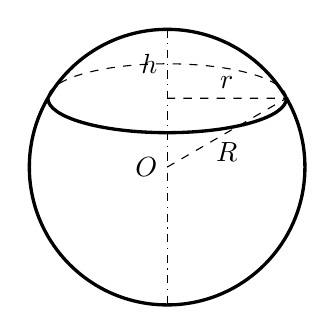
\begin{tikzpicture}[scale=1.75]
\draw[very thick](0,0) circle (1);
\draw[dashdotted](0,1)--(0,-1);  
\draw[very thick](1.732/2,.5) arc [start angle =0, end angle=-180, x radius=1.732/2, y radius=.25];
\draw[dashed](1.732/2,.5) arc [start angle =0, end angle=180, x radius=1.732/2, y radius=.25];
\draw[dashed](0,0)node[left]{$O$}--node[below]{$R$}(1.732/2,.5)--node[above]{$r$}(0,.5);
\node at (0,.75)[left]{$h$};


\end{tikzpicture}
\captionof{figure}{}
\end{minipage}

\begin{proof}
设截得这球冠的球的半径是$R$，则
\[r^2=(2R-h)h\]

$\therefore\quad r^2+h^2=2Rh$, 代入球冠面积公式$S_{\text{球冠}}=2\pi Rh$，得
\[S_{\text{球冠}}=\pi (r^2+h^2)\]
\end{proof}

球面夹在两个平行截面间的部分叫做\textbf{球带}，截得的两个圆叫做球带的\textbf{底}，这两个平行截面的距离叫做球带的\textbf{高}.

因为球带可以看作两个球冠的差，容易得到下述定理.

\begin{thm}
    {定理}球带的面积等于截成它的球的大圆周长与它的高的积.
即
\[S_{\text{球带}}=2\pi Rh\]
\end{thm}

\noindent
\begin{minipage}{.45\textwidth}
\centering
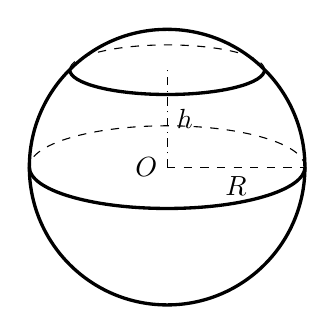
\begin{tikzpicture}[scale=1.75]
\draw[very thick](0,0) circle (1);
\draw[dashdotted](0,0)--node[right]{$h$}(0,.707);  
\draw[very thick](.707,.707) arc [start angle =0, end angle=-180, x radius=.707, y radius=.18];
\draw[dashed](.707,.707) arc [start angle =0, end angle=180, x radius=.707, y radius=.18];
\draw[dashed](0,0)node[left]{$O$}--node[below]{$R$}(1,0);

\tkzDrawPoint(0,0)
\tkzDrawPoint(0,.707)
\draw[very thick](1,0) arc [start angle =0, end angle=-180, x radius=1, y radius=.3];
\draw[dashed](1,0) arc [start angle =0, end angle=180, x radius=1, y radius=.3];


\end{tikzpicture}
\captionof{figure}{}
\end{minipage}
\hfill
\begin{minipage}{.45\textwidth}
\centering
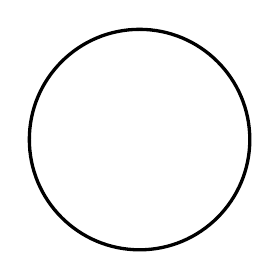
\begin{tikzpicture}[scale=1.4]
    \draw[very thick](0,0) circle (1);
  \tkzDefPoints{0/2/P,0/1/D, 0/0/O, 0/.5/C, .866/.5/B, -.866/.5/A}
\tkzDrawSegments[very thick](P,A P,B P,O A,B A,O B,O)
\tkzLabelPoints[left](A)
\tkzLabelPoints[right](B)
\tkzLabelPoints[above](P)
\tkzLabelPoints[above right](D)
\tkzLabelPoints[below right](C,O)

\end{tikzpicture}
\captionof{figure}{}
\end{minipage}



\begin{example}
    将地球近似地当作一个球，求人在宇宙飞船上，距地面4000公里高度时，能看到地球表面部分的面积（地球半径约为6370km）．
\end{example}

\begin{analyze}
在空中能看到的地球表面的部分是一个球冠. 要求它的面积，只要求出它的高. 这个高的大小只与$P$点的高低有关（因为地球的半径是定值）. 作出球的含有$P$点的轴截面，就容易求出这球冠的高.
\end{analyze}

\begin{solution}
人在宇宙飞船中离地面4000公里高度时，能看到地球表面的图形是球冠.

过飞船$P$和地球球心$O$的连线作地球的轴截面（图2.81）得到地球的大圆，$PA$、$PB$是这个圆的切线，$PD$是飞船$P$到
地球球面的距离，$CD$是能见到的地球球冠的高，$PD=4000$(km).

$\because\quad OA\bot PA,\quad AB\bot PO$,

$\therefore\quad OA^2=OC\cdot OP$,
\[\begin{split}
    \therefore\quad OC&=\frac{OA^2}{OP}=\frac{R^2}{R+PO}\\
    CD&=R-OC=R-\frac{R^2}{R+PD}=\frac{R\cdot PD}{R+PD}
\end{split}\]
\[\begin{split}
    \therefore\quad S_{\text{球冠}ADB}=2\pi R\cdot CD&=\frac{2\pi R^2\cdot PD}{R+PO}\\
&=\frac{2\x3.1416\x6370^2\x4000}{6370+4000}\\
&\approx 9.8\x10^7\; ({\rm km}^2)
\end{split}\]

答：能看到地球部分的面积为$9.8\x10^7$平方公里.
\end{solution}

\begin{example}
    在半径为$R$的球内，作一个内接等边圆柱，求球面被这圆柱的两底面截得的球冠和球带的面积.
\end{example}

\begin{analyze}
    这是求球冠高的问题. 求的方法还是要作出轴截
面.
\end{analyze}

\begin{solution}
作这个几何 体的 轴截面，得到的图形是一个半径为$R$的圆有一内接正方形如图2.82．

\noindent
\begin{minipage}{.7\textwidth}\CTEXindent
    作$OC\bot AB$于$C$，则所求球冠的高是$R-OC$，而所求球带的高是$2OC$．

    $\because\quad AB=\sqrt{2}R,\quad OC=\frac{\sqrt{2}}{2}R$
    
    $\therefore\quad $球冠的高$h_1=R-\frac{\sqrt{2}}{2}R$, 球带的高$h_2=\sqrt{2}R$.
\end{minipage}
\hfill
\begin{minipage}{.28\textwidth}
\centering
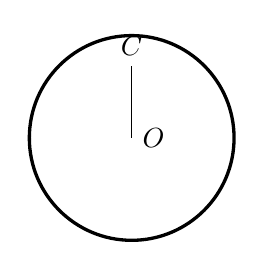
\begin{tikzpicture}[scale=1.3]
\draw[very thick](0,0)node[right]{$O$} circle(1);
\tkzDefPoint(45:1){B}
\tkzDefPoint(45+90:1){A}
\tkzDefPoint(-45:1){C'}
\tkzDefPoint(-45-90:1){D}
\tkzDrawPolygon[very thick](A,B,C',D)
\draw(0,0)--(0,.707)node[above]{$C$};
\tkzLabelPoints[left](A)
\tkzLabelPoints[right](B)
\end{tikzpicture}
\captionof{figure}{}
\end{minipage}
\[\begin{split}
    \therefore\quad S_{\text{球带}}&=2\pi Rh_2=2\pi R\cdot \sqrt{2}R=2\sqrt{2}\pi R^2\\
S_{\text{球冠}}&=\frac{1}{2}(S_{\text{球}}-S_{\text{球带}})
=\frac{1}{2}\left(4\pi R^2-2\sqrt{2}\pi R^2\right)
=\left(2-\sqrt{2}\right)\pi R^2
\end{split}\]
（或$S_{\text{球冠}}=2\pi R \left(R-\frac{\sqrt{2}}{2}R\right)=\left(2-\sqrt{2}\right)\pi R^2$   ）

答：所求球带的面积是$2\sqrt{2}\pi R^2$，两底截得的两个小球冠每个面积是$(2-\sqrt{2})\pi R^2$.
\end{solution}

\begin{remark}
通过本节例题的解法，可以看到作出轴截面的重要性.
\end{remark}

\subsection*{2.6  练习5}
一、选择题：
\begin{enumerate}
    \item 两个半径相等的球，每个球的球面通过另一个球的球心，则两球面在两球内的部分与其余部分面积的比是\hfill (\qquad )
\begin{multicols}{4}
\begin{enumerate}[(A)]
\item $ 1:4$.
    \item $1:3$.
    \item $1:2$.
    \item $3:16$.
\end{enumerate}    
\end{multicols}

\item 要使从一点发出的光能照亮半径为$r$的球的球面积的$\frac{1}{3}$, 那么这点光源与球心的距离为\hfill (\qquad )
\begin{multicols}{4}
    \begin{enumerate}[(A)]
\item $2r$.
\item $3r$.
\item $4r$.
\item $5r$.
    \end{enumerate}    
    \end{multicols}

\item 球冠形降落伞，其底面半径为$r$，高为$h$，降落伞的面积为\hfill (\qquad )
\begin{multicols}{2}
\begin{enumerate}[(A)]
\item $2\pi rh$.
\item $\pi h^2+\pi r^2$.
\item $\pi rh$
\item 不是以上答案.
\end{enumerate}    
\end{multicols}

\item 球冠的底面半径是球的半径的$\frac{1}{2}$，球冠与球面的面积的比是\hfill (\qquad )
\begin{multicols}{4}
\begin{enumerate}[(A)]
    \item $\frac{\sqrt{3}}{4}$
    \item $\frac{2-\sqrt{3}}{8}$
    \item $\frac{2-\sqrt{3}}{4}$
    \item $\frac{2-\sqrt{3}}{2}$
\end{enumerate}    
\end{multicols}

\item 球带的两底半径分别为20cm、24cm，球的半径为25cm，则球带的面积为\hfill (\qquad )
\begin{multicols}{2}
\begin{enumerate}[(A)]
\item $400\pi {\rm cm^2}$.
\item $1100\pi {\rm cm^2}$.
\item $200\pi {\rm cm^2}$.
\item $400\pi {\rm cm^2}$或$1100\pi {\rm cm^2}$．
\end{enumerate}    
\end{multicols}
\end{enumerate}

二、填空题：
\begin{enumerate}
\item 已知球冠的底面半径是$r$，高是$h$，那么截得这球冠的球的半径$R=$\blank
\item 已知球的半径是$R$，它的一个球冠面积是球的面积的$\frac{2}{3}$，这球冠的高是\blank.
\item 半径为$R$的$120^{\circ}$弧，绕过弧中点的直径旋转所得球冠的面积是\blank.
\item 地球北温带的面积是\blank．（地球半径约6370km，北回归线是北纬$23.5^{\circ}$，北极圈
是北纬$66.5^{\circ}$）．
\item 地球的半径是$R$，卫星离地面高度为$h$时，可观测地面表面积为$S$，则$S$和$h$的函数关系是\blank.
\item 球冠的底面半径是球半径的$\frac{1}{2}$，那么球冠与球的面积的比是\blank.
\item 已知球的半径是25cm，一个不过球心的截面面积等于$49\pi {\rm cm^2}$，则球心到这个截面的距离是\blank，这个截面截球所得的球冠面积是\blank.
\item 举出在日常生活中，你见到的球冠的实例。
\end{enumerate}

\section*{习题五}
\begin{center}
    \bfseries A
\end{center}

\begin{enumerate}
\item 在半径是13cm的球面上有$A$、$B$、$C$三点，$AB=6$cm, $BC=8$cm, $CA=10$cm，求经过这三点的截面和球心$O$的距离.
\item 在半径是$R$的球面上有两点$A$、$B$，半径$OA$和$OB$的夹角是$\theta$ ($\theta<180^{\circ}$)，求$A$、$B$两点间的球面距离.
\item 我国第一颗人造地球卫星的远地点距地面2384km，在这时，地球上有多少平方公里上的人能看到这颗卫星？
\item 在半径为$R$的球内，作一内接等边圆柱，求球面被这圆柱的两底面截得的球冠和球带的面积.
\item 半径为$R$的四个球，每一个都和其它三个相切，求和这四个球同时相切的球的半径.
\item 在半径为30cm的球面上有三个点，它们间的距离分别是20cm，12cm，16cm．求这三点所在平面截球面所得较大的球冠面积。
\end{enumerate}

\begin{center}
    \bfseries B
\end{center}
\begin{enumerate}\setcounter{enumi}{6}
\item 在半径为$R$的球中，钻一个圆锥形孔，使圆锥的顶点在球面上，其轴通过球心，母线与轴成$\alpha$角，求球挖去圆锥后，所形成的几何体的表面面积.
\item 一个圆锥的高为$\frac{32}{3}$cm，它的侧面展开图的圆心角是$216^{\circ}$.
\begin{enumerate}[(1)]
\item 求此圆锥的底面半径和母线长；
\item 间距底面多远的平行截面，截得的圆台有内切球？
\item 求（2）中圆台的侧面积。
\end{enumerate}
\end{enumerate}

\begin{center}
    \bfseries C
\end{center}
\begin{enumerate}\setcounter{enumi}{8}
\item 半径为$r_1$的球$O_1$内切于圆锥，半径为$r_2\; (r_2<r_1)$的球$O_2$与球$O_1$外切且与圆锥内侧面内切，两过切点且平行于底面的平面截这圆锥，求所得圆台的侧面积。
\item 地球半径为$R$，地面上两点$A$、$B$都在北纬$\alpha$度圈上，经度相差$\beta$度，求$A$、$B$两点间的球面距离.
\item 圆锥的内切半球的大圆在圆锥的底面上，已知$S_{\text{圆锥全}}:S_{\text{半}}=18:5$，求圆锥的顶角.   
\end{enumerate}


